\newcommand\operatorKey[1]{
  \begin{center}
    \includegraphics[height=10mm]{images/#1}
  \end{center}
  }

\chapter{Reference}

\section{Tabs}

\emph{Ravel} has six Tabs:
\begin{itemize}
\item \emph{Wiring}, which houses the Operators and the Design canvas on
which data analysis (\emph{Ravel}) and dynamic models (\emph{Minsky})
are constructed;
\item \emph{Equations}, which shows the equations created by the analysis
or model on the Wiring Tab;
\item \emph{Summary}, which shows a hierarchical overview of all the definitions
of variables and parameters in the model;
\item \emph{Phillips Diagram}, a \emph{Minsky}-specific view of the financial
flows in a dynamic economic model;
\item \emph{Publication}, which enables selected items from a Wiring to
be displayed; and
\item +, which adds additional Publication Tabs
\end{itemize}

\subsection{Wiring}

The Wiring Tab consists of:
\begin{itemize}
\item The \htmlref{Operations bar}{Operations}, which contains all of \emph{Ravel}'s
mathematical operators; and
\item The design canvas, a free-form space on which variables, parameters
and operations are combined to perform analysis of data in \emph{Ravel},
and to simulate dynamic systems in \emph{Minsky}.
\end{itemize}

\subsection{Equations}

The Equation Tab shows the equations in your data analysis or model.
To export equations in a format that can be inserted into \LaTeX{} editors
or programs like MathType, choose ``Export canvas as'' from the
File menu, and choose the format LaTeX. For details see \htmlref{\emph{Working with Other Programs}}{Export}.

\subsection{Summary}

The Summary Tab shows the equations in your data analysis or model
in a structured tabular layout. For details see \htmlref{\emph{Summary
    tab}}{tabs:Summary}.

\subsection{Phillips Diagram}

\label{tabs:Phillips}

This tab implement's Minsky's take on a \htmladdnormallink{Phillips
  diagram showing the stocks and flows in a monetary
  economy}{https://en.wikipedia.org/wiki/Phillips_Machine}. The
Phillips tab shows all the information contained in the Godley tables
of the model - if there aren't any, this tab will be blank.

\subsection{Publication }

\label{tabs:Publication}

A Publication Tab enables you to place any item on the Wiring canvas
in any location. This is useful for distributing the results of a
model without having to show all the workings involved in deriving
results.

Any item from the wiring tab can be added to a publication tab, and
then moved, resized or rotated independently of the item on the wiring
tab. To add an item to a Publication Tab, hover the mouse over the
item and choose ``Add item to a publication tab'' from the context
menu. The sub-menu lists available Publication tabs. Click on the
one you wish to place the item on, and the item will be placed in
the upper-left hand corner of that tab. It can then be moved to anywhere
else on that tab.

For items that dynamically update, the publication tab will be updated
dynamically when selections on the Wiring Tab are altered.

\emph{Ravel} components can also be manipulated on the Publication
tab--for example, a different store can be selected on the ``Store''
axis of a Ravel documenting retail sales. If a Ravel has a caliper
applied to an axis on the Wiring Tab, to, for example, select a range
of dates, that caliper can be moved to a different range of dates
on the Publication Tab.

Textual annotation can be added to the publication tab, independently
of any annotations on the wiring tab.

Wires currently cannot be added to the publication tab. However, you
can insert text-based arrows (eg $\rightarrow$) by typing \verb+#\rightarrow+
on the canvas. This item can then be rotated and scaled to emulate the wiring
diagram connecting parts of the dashboard together.

\section{Operations}

\label{Operations}

\noindent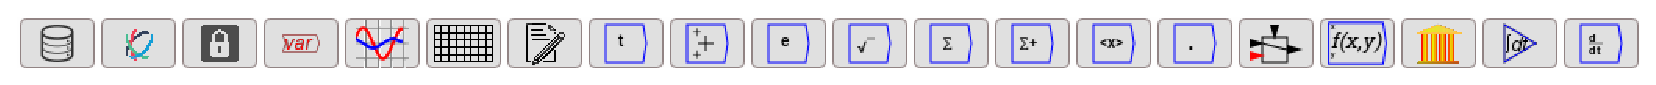
\includegraphics[width=\textwidth]{images/DesignIcons}

Except for \buttonIcon{var}, which invokes a pop-up sideways
menu for defining variables, constants and parameters, the first 8
icons on the Operations bar---from data importing to the simulation
time--are immediately activated by clicking on them. The remaining
mathematical and data operations are stored on pop-up sideway menus,
which are activated when you click on the menu's icon. For example,
clicking on the \buttonIcon{Plus} symbol brings up the
Binary Operators menu:

\noindent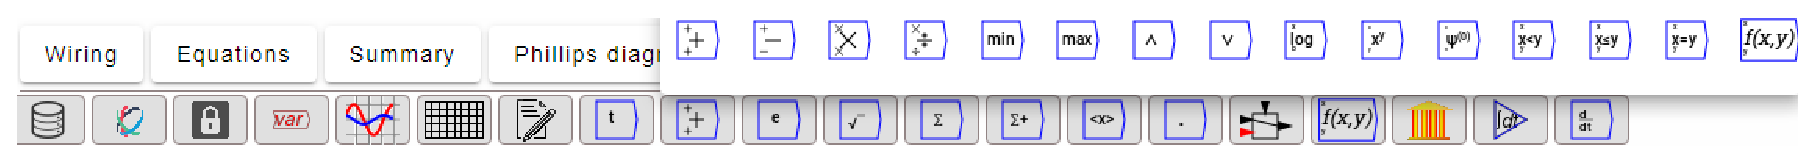
\includegraphics[width=\textwidth]{images/DesignIconsWithBinaryOperatorsMenu}

\subsection{Import Data}

The import data operator \buttonIcon{importData} inserts
a parameter on the canvas called \buttonIcon{dataImport},
and invokes the data import form. For more details see \htmlref{CSV import}{CSV import}.

\subsection{Ravel}

A Ravel is a visual tool for manipulating and analyzing multi-dimensional
data. For full details on the concept see \htmlref{Ravel}{Ravel}.

The Ravel operator \buttonIcon{ravelIcon}inserts a
Ravel onto the Wiring canvas. The first Ravel inserted is in Edit
mode, and has sample axis names and a sample data point selected.

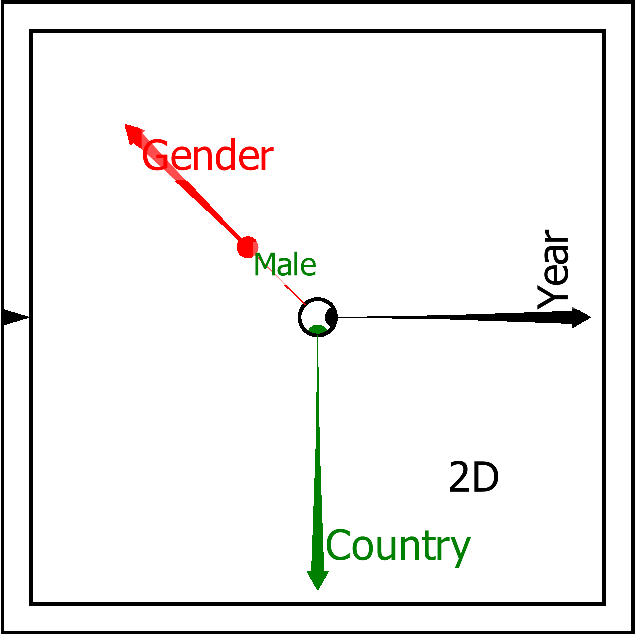
\includegraphics[width=10cm]{images/RavelBlank}

Subsequent Ravels are inserted in iconized mode.

%
\includegraphics{images/RavelIcon}

To use a Ravel, it must first have a parameter (or variable) attached
to it. Normally the parameter will contain data imported from a CSV
file---for more details see \htmlref{CSV import}{CSV import}.

The key feature of a Ravel is its Axes (or ``Arrows''). A Ravel
has one axis per dimension of the data attached to it. Axes can be:
\begin{description}
\item[Rotated] The right-pointing axis determines what is shown on
the x-axis of a Plot and columns of a Sheet; the down-pointing axis
determines what is displayed on the Y-axis of a plot and the rows
of a sheet.
\item[Collapsed] An axis is collapsed by dragging the arrow head
back to the centre of the Ravel. This applies an aggregation method
to the axis, which is determined by the setting for ``Set next aggregation''
on the context menu. The aggregations are Sum, Product, Average, Standard
Deviation, Maximum and Minimum. The aggregation type can be changed
{\em post facto} unser the ``Axis properties'' context menu. 
\item[Selected] When the selector dot for an Axis is in the centre
of the Ravel, the entire Ravel axis is output (though this can be a selection
of values on the axis if ``Pick axis slices'' has been activated).
When the selector dot is on a particular value on an axis, only that
value is output.
\item[Sorted] The ``none'' sort order of a Ravel is that of
the axis as it is attached (usually the order in which it is read from
a CSV file). The axis can also be sorted in
either a ``forward'' or ``reverse''  direction. The sorting comparison
depends on the dimension type --- numerical in the case of ``value'',
time order in the case of ``time'' and {\em lexicographic}
(``alphabetical'') in the case of ``string''.
\item[Sorted by value] When the output of a Ravel is 1-dimensional,
axes can be sorted by the data values along this 1-dimensional axis.
The choices are a combination of Forward and Reverse, and Statically
and Dynamically. A Static sort applies the order of the data for a
given instance---for example, countries could be sorted by the inflation
rate for 2022. This sort order is maintained if the selector dot for
date is altered. For example, with a static sort, choosing 2000 on
the Date axis would show the inflation rate in 2000, with countries
sorted according to their inflation rates in 2022. A Dynamic sort
applies the sort order for each selection. For example, a reverse
dynamic sort of Country by inflation rates would show countries by
descending order of their inflation rate in whichever year was chosen
on the Date axis.
\item[Picked] The context menu option ``Pick axis slices'' invokes
a pop-down menu showing all the entries on that axis---countries
for a Country axis, dates for a Time axis, etc. You can select specific
values by clicking on them, and select multiple values by control-clicking
on them.
\item[Calipered] ``Toggle axis calipers'' brings up a caliper which
initially spans the entire data range. The ends of the caliper can
be individually adjusted to select a range of the data, while the
whole caliper can be moved to select the same number of data points
for different segments of the data.
\end{description}
Ravels can be linked with other Ravels that share the same dimension(s).
This means that any operation applies to one Ravel is applied to all
Ravels in the linked set. For more details see \htmlref{\emph{Linking Ravels}}{Linking-Ravels}.

\subsection{Lock}

\begin{center}
  
\includegraphics{images/Lock}
\end{center}

Locks are attached to the output of Ravels. After a Lock is closed
(either by double-clicking on the Lock, or choosing Lock from the
context menu), alterations can be made to the source Ravel without
altering the output of the Lock. This makes it possible to take multiple
slices of the data from one Ravel, and to assign those slices to variables
so that they can be further analyzed by \emph{Ravel}. For details
see \htmlref{\emph{Lock}}{Lock}

\subsection{Variable}

\begin{center}
  
\includegraphics{images/var}
\end{center}
    
This operator activates a pop-up menu for defining variables, parameters
and constants. For details see \htmlref{\emph{Variables}}{Variables}.

\subsection{Plot}
\begin{center}
  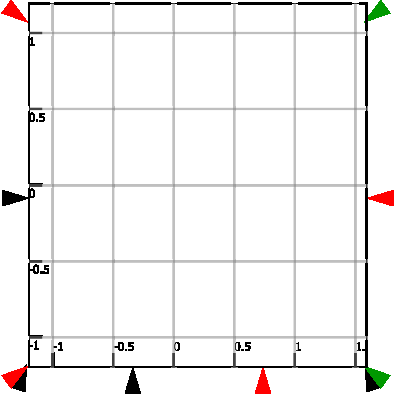
\includegraphics{images/plot}
\end{center}

This operator inserts a Plot onto the Wiring canvas. For details see
\htmlref{\emph{Plot Widget}}{PlotWidget}.

\subsection{Sheet}
\begin{center}
  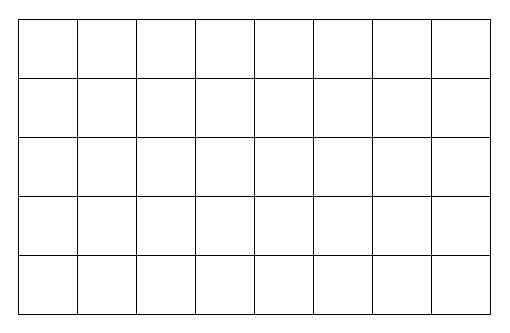
\includegraphics{images/sheet}
\end{center}

This operator inserts a Sheet onto the Wiring canvas. For details
see \htmlref{\emph{Sheet}}{Sheet}.

\subsection{time $t$}
\operatorKey{time}

\label{Operation:time} Returns the current value of system time.

The operator can be placed on the canvas in two ways:
\begin{itemize}
\item From the time widget on the toolbar \buttonIcon{time};
or 
\item By typing the letters "time" on the canvas and then pressing the
Enter key.
\end{itemize}

\subsection{Binary Operations}

\label{Binary-Operations}\label{operations-binop}

\subsubsection{add +}

\operatorKey{PlusSymbol}

\label{Operation:add} Add multiple numbers together.

The input ports allow multiple wires, which are all summed. If an
input port is unwired, it is equivalent to setting it to zero.

The operator can be placed on the canvas in two ways:
\begin{itemize}
\item From the \emph{Binary Operations (``binop'') }toolbar; or 
\item By pressing the plus key anywhere on the wiring canvas. 
\end{itemize}

\subsubsection{subtract $-$}

\operatorKey{MinusKey}

\label{Operation:subtract} Subtract two numbers. The input ports
allow multiple wires, which are summed prior to the subtraction being
carried out. If an input port is unwired, it is equivalent to setting
it to zero. Note the small `+' and `$-$' signs on the input ports
indicating which terms are added or subtracted from the result.


The operator can be placed on the canvas in two ways:
\begin{itemize}
\item From the \emph{Binary Operations (``binop'')} toolbar; or 
\item By pressing the minus key anywhere on the wiring canvas, \textit{followed
by pressing the Enter key, or clicking on OK in the text input window}.
The reason for requiring the Enter key to be pressed---rather than
immediately placing the minus operator on the keyboard, as with the
plus and multiply operators---is that a user may wish to enter a
negative number as a constant. 
\end{itemize}

\noindent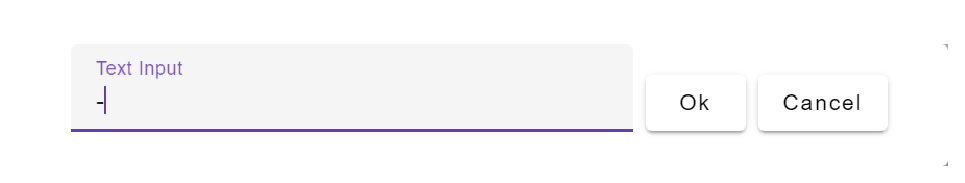
\includegraphics[width=\textwidth]{images/MinusTextWindow}

\subsubsection{multiply $\times$}

\operatorKey{MultiplyKey}

\label{Operation:multiply} Multiply numbers with each other. The
input ports allow multiple wires, which are all multiplied together.
If an input port is unwired, it is equivalent to setting it to one.


The operator can be placed on the canvas in two ways:
\begin{itemize}
\item From the \emph{Binary Operations (``binop'')} toolbar; or 
\item By pressing the multiply (asterisk: {*}) key anywhere on the wiring
canvas. 
\end{itemize}

\subsubsection{divide $\div$}

\operatorKey{DivideKey}

\label{Operation:divide} Divide a number by another. The input ports
allow multiple wires, which are multiplied together for each port
prior to the division being carried out. If an input port is unwired,
it is equivalent to setting it to one. Note the small `$\times$'
and `$\div$' signs indicating which port refers to the numerator
and which the denominator.

The operator can be placed on the canvas in two ways:
\begin{itemize}
\item From the \emph{Binary Operations (``binop'')} toolbar; or 
\item By pressing the divide key (/) anywhere on the wiring canvas. 
\end{itemize}

\subsubsection{min}

\operatorKey{minkey}

\label{Operation:min} Returns the minimum of $x$ and $y$. If multiple
wires are connected to the ports, the the overall minimum from all
inputs is returned.

The operator can be placed on the canvas in two ways:
\begin{itemize}
\item From the \emph{Binary Operations (``binop'')} toolbar; or 
\item By typing the letters ``min'' on the canvas and then pressing the
Enter key. 
\end{itemize}

\subsubsection{max}

\operatorKey{maxkey}

\label{Operation:max} Returns the maximum of $x$ and $y$. If multiple
wires are connected to the ports, the the overall maximum from all
inputs is returned.

The operator can be placed on the canvas in two ways:
\begin{itemize}
\item From the \emph{Binary Operations (``binop'') }toolbar; or 
\item By typing the letters "max" on the canvas and then pressing the
Enter key. 
\end{itemize}

\subsubsection{and $\wedge$}

\operatorKey{andkey}

\label{Operation:and_} Logical and of $x$ and $y$, where $x\le0.5$
means false, and $x>0.5$ means true. The output is 1 or 0, depending
on the result being true (1) or false (0) respectively.

The operator can be placed on the canvas in two ways:
\begin{itemize}
\item From the \emph{Binary Operations (``binop'') }toolbar; or 
\item By typing the letters "and\_" (the word and, \emph{followed by an
underscore}) on the canvas and then pressing the Enter key. The underscore
is needed because ``and'' is a reserved word in \emph{C++,} the
programming language in which \emph{Ravel} is written.
\end{itemize}

\subsubsection{or $\vee$}

\operatorKey{or}

\label{Operation:or_} Logical or of $x$ and $y$, where $x\le0.5$
means false, and $x>0.5$ means true. The output is 1 or 0, depending
on the result being true (1) or false (0) respectively.

The operator can be placed on the canvas in two ways:
\begin{itemize}
\item From the \emph{Binary Operations (``binop'') }toolbar; or 
\item By typing the letters ``or\_'' (the word or, \emph{followed by an
underscore}) on the canvas and then pressing the Enter key. The underscore
is needed because ``or'' is a reserved word in \emph{C++,} the programming
language in which \emph{Ravel} is written.
\end{itemize}

\subsubsection{log}

\operatorKey{LogKey}

\label{Operation:log} Take the logarithm of the $x$ input port,
to base $b$. The base $b$ needs to be specified --- if the natural
logarithm is desired ($b=e$), use the \htmlref{natural log}{Operation:ln} instead.

The operator can be placed on the canvas in two ways:
\begin{itemize}
\item From the \emph{Binary Operations (``binop'')} toolbar; or 
\item By typing the word ``log'' anywhere on the wiring canvas, and then
pressing the Enter key. 
\end{itemize}
When you use the direct typing method to enter the Log operator, the
text entry window pops up. This allows you to type a variable/parameter
name starting with Log (like, for example, ``Logical''. If you press
Enter (or click on OK) with only the word Log in the window, the Log
operator will be placed on the canvas.

\subsubsection{pow $x^{y}$}

\operatorKey{PowerKey}

\label{Operation:pow} Raise one number to the power of another. The
ports are labelled $x$ and $y$, referring the the formula $x^{y}$.

The operator can be placed on the canvas in two ways:
\begin{itemize}
\item From the \emph{Binary Operations (``binop'')} toolbar; or 
\item By typing the letters ``Pow'' anywhere on the wiring canvas and then
pressing the Enter Key (or clicking on OK). 
\end{itemize}

\subsubsection{Polygamma $\psi^{(n)}(x)$}

\operatorKey{Polygamma}

\label{Operation:polygamma} Returns the polygamma function of the
first argument $x$, with the order $n$ being given by the floor
of the second argument. 
\[
\psi^{(n)}(x)=\frac{d^{n+1}}{dx^{n+1}}\ln\Gamma(x)
\]

The operator can be placed on the canvas in two ways:
\begin{itemize}
\item From the \emph{Binary Operations (``binop'')} toolbar; or 
\item By typing the letters ``polygamma'' on the canvas and then pressing
the Enter key.
\end{itemize}

\subsubsection{lt $<$}

\operatorKey{LessThanKey}

\label{Operation:lt} Returns 0 or 1, depending on whether $x<y$
is true (1) or false (0).

The operator can be placed on the canvas in two ways:
\begin{itemize}
\item From the \emph{Binary Operations (``binop'')} toolbar; or 
\item By typing the letters "lt" on the canvas and then pressing the Enter
key. 
\end{itemize}

\subsubsection{le $\le$}

\operatorKey{LessEqualKey}

\label{Operation:le} Returns 0 or 1, depending on whether $x\le y$
is true (1) or false (0).

The operator can be placed on the canvas in two ways:
\begin{itemize}
\item From the \emph{Binary Operations (``binop'')} toolbar; or 
\item By typing the letters "le" on the canvas and then pressing the Enter
key. 
\end{itemize}

\subsubsection{eq $=$}

\operatorKey{Equal}

\label{Operation:eq} Returns 0 or 1, depending on whether $x=y$
is true (1) or false (0).

The operator can be placed on the canvas in two ways:
\begin{itemize}
\item From the \emph{Binary Operations (``binop'')} toolbar; or 
\item By typing the letters ``eq'' on the canvas and then pressing the Enter
key. 
\end{itemize}

\subsection{Special constants}

\label{Special-constants}\label{operations-constop}

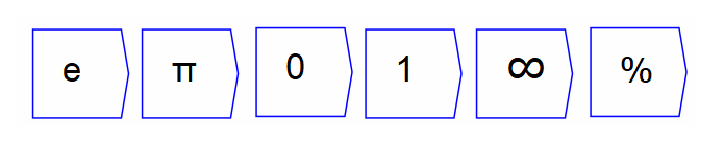
\includegraphics{images/FundamentalConstants}

\label{Operation:euler}\label{Operation:pi}\label{Operation:zero}\label{Operation:one}
\label{Operation:inf}

Some special constants ($e=2.72\ldots$, $\pi=3.14\ldots$, 0, 1,
$\infty$) can be placed on the canvas, via two methods:
\begin{itemize}
\item By clicking on the relevant icon on the \emph{Fundamental Constants
(``constop'')} toolbar; or 
\item By typing the constant name on the canvas, and pressing Enter (or
clicking OK) in the variable definition window. These names are: \textit{Euler}
for $e=2.72\ldots$; \textit{pi} for $\pi=3.14\ldots$; \textit{inf}
for $\infty$; and the percent symbol for the percent operator (which
multiplies the input by 100).
\end{itemize}

\subsubsection{Percent}

\operatorKey{PercentOperator}

\label{Operation:percent} The percent operator takes one input, and
multiplies its elements by 100. It is useful for converting fractions
into percentages for display purposes.

The operator can be placed on the canvas in two ways:
\begin{itemize}
\item From the \emph{Fundamental Constants (``constop'')} toolbar; or 
\item By pressing the percent key anywhere on the wiring canvas. 
\end{itemize}

\subsection{Functions/Unary Operators}

\label{Functions/Unary-Operators}\label{operations-function}

\subsubsection{sqrt $\protect\surd$}

\operatorKey{squareRoot}
    
\label{Operation:sqrt} This produces the square root of the input
value.

For example, connecting the value of 9 with the ``sqrt'' block will
produce the value of 3. As with all Ravel operators, this function
accepts multidimensional arguments.

The operator can be placed on the canvas in two ways:
\begin{itemize}
\item From the \emph{Functions (``function'')} toolbar; or 
\item By typing the letters ``sqrt'' on the canvas and then pressing the
Enter key. 
\end{itemize}

\subsubsection{exp}

\operatorKey{Exponential}

\label{Operation:exp} Connecting a variable (for example, ``time'')
to this block will produce the exponential function $e^{x}$ where
x is the input variable.

The operator can be placed on the canvas in two ways:
\begin{itemize}
\item From the \emph{Functions (``function'')} toolbar; or 
\item By typing the letters ``exp'' on the canvas and then pressing the
Enter key. 
\end{itemize}

\subsubsection{ln}

\operatorKey{ln}

\label{Operation:ln} Produces a natural logarithm of the input, to
the base of e. This takes the equation $\log_{e}x$ where $x$ is
the input.

The operator can be placed on the canvas in two ways:
\begin{itemize}
\item From the \emph{Functions (``function'')} toolbar; or 
\item By typing the letters ``ln'' on the canvas and then pressing the Enter
key. 
\end{itemize}

\subsubsection{sin}

\operatorKey{sine}

\label{Operation:sin} Produces a sine function of the input.

For example, connecting a ``time'' block to this function, and then
to a graph, will produce a sine wave.

The operator can be placed on the canvas in two ways:
\begin{itemize}
\item From the \emph{Functions (``function'')} toolbar; or 
\item By typing the letters ``sin'' on the canvas and then pressing the
Enter key. 
\end{itemize}
For further explanation regarding trigonemtric functions, see
\htmladdnormallink{Wikipedia's page on trigonometric functions}{https://en.wikipedia.org/wiki/Trigonometric_functions}.

\subsubsection{cos}

\label{Operation:cos} Produces a cosine function of the input.

\operatorKey{cosine}

The operator can be placed on the canvas in two ways:
\begin{itemize}
\item From the \emph{Functions (``function'')} toolbar; or 
\item By typing the letters ``cos'' on the canvas and then pressing the
Enter key.
\end{itemize}
For example, connecting a ``time'' block to this function, and then
to a graph, will produce a cosine wave. For further explanation regarding
trigonemtric functions, see \htmladdnormallink{Wikipedia's page on trigonometric functions}{https://en.wikipedia.org/wiki/Trigonometric_functions}.

\subsubsection{tan}

\operatorKey{tan}

\label{Operation:tan} Produces a tangent function of the input.

The operator can be placed on the canvas in two ways:
\begin{itemize}
\item From the \emph{Functions (``function'')} toolbar; or 
\item By typing the letters ``tan'' on the canvas and then pressing the
Enter key.
\end{itemize}
For example, connecting a ``time'' block to this function, and then
to a graph, will produce a tangent graph. For further explanation
regarding trigonemtric functions, see \htmladdnormallink{Wikipedia's page on trigonometric functions}{https://en.wikipedia.org/wiki/Trigonometric_functions}.

\subsubsection{asin}

\operatorKey{sin-1}

\label{Operation:asin} Produces an arc sine function of the input,
or the inverse of the sine function.

The operator can be placed on the canvas in two ways:
\begin{itemize}
\item From the \emph{Functions (``function'')} toolbar; or 
\item By typing the letters ``asin'' on the canvas and then pressing the
Enter key.
\end{itemize}
For further explanation regarding trigonemtric functions, see \htmladdnormallink{Wikipedia's page on trigonometric functions}{https://en.wikipedia.org/wiki/Trigonometric_functions}.

\subsubsection{acos}

\operatorKey{cos-1}

\label{Operation:acos} Produces an arc cosine function of the input,
or the inverse of the cosine function.

The operator can be placed on the canvas in two ways:
\begin{itemize}
\item From the \emph{Functions (``function'')} toolbar; or 
\item By typing the letters ``acos'' on the canvas and then pressing the
Enter key.
\end{itemize}
For further explanation regarding trigonemtric functions, see \htmladdnormallink{Wikipedia's page on trigonometric functions}{https://en.wikipedia.org/wiki/Trigonometric_functions}.

\subsubsection{atan}

\operatorKey{tan-1}

\label{Operation:atan} Produces an arc tangent function of the input,
or the inverse of the tangent function.

The operator can be placed on the canvas in two ways:
\begin{itemize}
\item From the \emph{Functions (``function'')} toolbar; or 
\item By typing the letters ``atan'' on the canvas and then pressing the
Enter key.
\end{itemize}
For further explanation regarding trigonemtric functions, see \htmladdnormallink{Wikipedia's page on trigonometric functions}{https://en.wikipedia.org/wiki/Trigonometric_functions}.

\subsubsection{sinh}

\operatorKey{sinh}

\label{Operation:sinh} hyperbolic sine function $\frac{e^{x}-e^{-x}}{2}$ 

The operator can be placed on the canvas in two ways:
\begin{itemize}
\item From the \emph{Functions (``function'')} toolbar; or 
\item By typing the letters ``sinh'' on the canvas and then pressing the
Enter key.
\end{itemize}

\subsubsection{cosh}

\operatorKey{cosh}

\label{Operation:cosh} hyperbolic cosine function $\frac{e^{x}+e^{-x}}{2}$ 

The operator can be placed on the canvas in two ways:
\begin{itemize}
\item From the \emph{Functions (``function'')} toolbar; or 
\item By typing the letters ``cosh'' on the canvas and then pressing the
Enter key.
\end{itemize}

\subsubsection{tanh}

\operatorKey{tanh}

\label{Operation:tanh} hyperbolic tangent function $\frac{e^{x}-e^{-x}}{e^{x}+e^{-x}}$ 

The operator can be placed on the canvas in two ways:
\begin{itemize}
\item From the \emph{Functions (``function'')} toolbar; or 
\item By typing the letters ``tanh'' on the canvas and then pressing the
Enter key.
\end{itemize}

\subsubsection{abs $|x|$}

\operatorKey{abs}

\label{Operation:abs} absolute value function. Returns the magnitude
of any entered variable.

The operator can be placed on the canvas in two ways:
\begin{itemize}
\item From the \emph{Functions (``function'')} toolbar; or 
\item By typing the letters ``abs'' on the canvas and then pressing the
Enter key.
\end{itemize}

\subsubsection{floor $\lfloor x\rfloor$}

\operatorKey{floor}

\label{Operation:floor} The greatest integer less than or equal to
$x$. 

The operator can be placed on the canvas in two ways:
\begin{itemize}
\item From the \emph{Functions (``function'')} toolbar; or 
\item By typing the letters ``floor'' on the canvas and then pressing the
Enter key.
\end{itemize}

\subsubsection{frac}

\operatorKey{frac}

\label{Operation:frac} Fractional part of $x$, ie $x-\lfloor x\rfloor$.

The operator can be placed on the canvas in two ways:
\begin{itemize}
\item From the \emph{Functions (``function'')} toolbar; or 
\item By typing the letters ``frac'' on the canvas and then pressing the
Enter key.
\end{itemize}

\subsubsection{not $\neg$}

\operatorKey{not}

\label{Operation:not_} The output is 1 or 0, depending on whether
$x\le0.5$ is true (1) or false (0) respectively.

The operator can be placed on the canvas in two ways:
\begin{itemize}
\item From the \emph{Functions (``function'')} toolbar; or 
\item By typing the letters ``not\_'' (the word not, \emph{followed by an
underscore}) on the canvas and then pressing the Enter key. The underscore
is needed because ``not'' is a reserved word in \emph{C++,} the
programming language in which \emph{Ravel} is written.
\end{itemize}

\subsubsection{Gamma $\Gamma$}

\operatorKey{Gamma}

\label{Operation:Gamma} Returns the Gamma function of its argument:
\[
\Gamma(x)=\int_{0}^{\infty}t^{x-1}e^{-t}dt
\]

The operator can be placed on the canvas in two ways:
\begin{itemize}
\item From the \emph{Functions (``function'')} toolbar; or 
\item By typing the letters ``gamma'' on the canvas and then pressing the
Enter key.
\end{itemize}

\subsubsection{Factorial !}

\operatorKey{Factorial}

\label{Operation:fact} Returns the factorial of its argument: 
\begin{eqnarray*}
0! & = & 1\\
n! & = & \prod_{i=1}^{n}i\\
\end{eqnarray*}

The operator can be placed on the canvas in two ways:
\begin{itemize}
\item From the \emph{Functions (``function'')} toolbar; or 
\item By typing the letters ``fact'' on the canvas and then pressing the
Enter key.
\end{itemize}
Note: 
\[
n!=\Gamma(n+1)
\]
which is how it is implemented in Minsky.

\emph{Minsky} provides this function because of its relationship to
the derivative of the Gamma function (and factorials).

\subsubsection{copy}\label{Operation:copy} This just copies its input to its output,
which is redundant on wiring diagrams, but is needed for internal
purposes.

\subsection{differentiate $d/dt$}\label{Operation:differentiate}
Symbolically differentiates its input with respect to system time,
producing d/dt[input].  For further explanation regarding
differentiation, see
\htmladdnormallink{this wikipedia page}{https://en.wikipedia.org/wiki/Derivative}.

\subsection{User defined
  function}\label{Operation:userFunction}\label{UserFunction}

A user defined function is a function defined by an algebraic
expression. Support for this feature is courtesy of the wonderful
\htmladdnormallink{exprtk}{http://www.partow.net/programming/exprtk/index.html}
library developed by Arash Partow.

A user defined function has a {\em name}, {\em parameters} and an {\em
  expression}. Example expressions are things like \verb'x+y' or
\verb'sin(x)'. More details of the sorts of expressions possible can
be found in the \htmlref{User Defined Functions}{ExprTk} section of
the manual.

The parameters are specified as part of the name, so a user defined
function adding x and y would be called \verb'useradd(a,y)' and the
sin example might be called \verb'mysin(x)'. Functions with up to two
arguments can be wired on the canvas. User defined functions can call
other user defined functions, so specifiying more than 2 parameters
can be a useful thing to do.

\subsection{Tensor operations}
\label{operations-reduction}\label{operations-scan}\label{operations-tensor}

\label{Operations: Reduction}

\subsubsection{sum $\sum$}

\operatorKey{sum}

\label{Operation:sum} Sum along a given axis.

The operator can be placed on the canvas in two ways:
\begin{itemize}
\item From the \emph{Reductions Operations (``reduction'')} toolbar \buttonIcon{sum};
or 
\item By typing the letters ``sum'' on the canvas and then pressing the
Enter key.
\end{itemize}
The same result can be achieved by collapsing the relevant Ravel axis
after choosing $\Sigma$ from the ``Set next
aggregation'' context menu.

\subsubsection{product $\prod$}

\operatorKey{product}

\label{Operation:product} Multiply along a given axis.

The operator can be placed on the canvas in two ways:
\begin{itemize}
\item From the \emph{Reductions Operations (``reduction'')} toolbar \buttonIcon{sum};
or 
\item By typing the letters ``product'' on the canvas and then pressing
the Enter key.
\end{itemize}
The same result can be achieved by collapsing the relevant Ravel axis
after choosing $\Pi$ from the ``Set next
aggregation'' context menu.

\subsubsection{infimum}

\operatorKey{infimum}

\label{Operation:infimum} Return the least value along a given axis.

The operator can be placed on the canvas in two ways:
\begin{itemize}
\item From the \emph{Reductions Operations (``reduction'')} toolbar \buttonIcon{sum};
or 
\item By typing the letters ``infimum'' on the canvas and then pressing
the Enter key.
\end{itemize}

\subsubsection{supremum}

\label{Operation:supremum} Return the greatest value along a given
axis.

\operatorKey{supremum}

The operator can be placed on the canvas in two ways:
\begin{itemize}
\item From the \emph{Reductions Operations (``reduction'')} toolbar \buttonIcon{sum};
or 
\item By typing the letters ``supremum'' on the canvas and then pressing
the Enter key.
\end{itemize}

\subsubsection{any}

\operatorKey{any}

\label{Operation:any} Return 1 if any value along a given axis is
nonzero, otherwise return 0 if all are zero.

The operator can be placed on the canvas in two ways:
\begin{itemize}
\item From the Reductions Operations toolbar \buttonIcon{sum};
or 
\item By typing the letters ``any'' on the canvas and then pressing the
Enter key.
\end{itemize}

\subsubsection{all}

\operatorKey{all}

\label{Operation:all} Return 1 if all values along a given axis are
nonzero, otherwise return 0 if any are zero.

The operator can be placed on the canvas in two ways:
\begin{itemize}
\item From the \emph{Reductions Operations (``reduction'')} toolbar \buttonIcon{sum};
or 
\item By typing the letters ``all'' on the canvas and then pressing the
Enter key.
\end{itemize}

\subsubsection{infindex}

\label{Operation:infIndex} Return the index of the least value along
a given axis.

\operatorKey{infindex}

The operator can be placed on the canvas in two ways:
\begin{itemize}
\item From the \emph{Reductions Operations (``reduction'')} toolbar \buttonIcon{sum};
or 
\item By typing the letters ``infIndex'' on the canvas and then pressing
the Enter key.
\end{itemize}

\subsubsection{supindex}

\label{Operation:supIndex} Return the index of the greatest value
along a given axis.

\operatorKey{supindex}

The operator can be placed on the canvas in two ways:
\begin{itemize}
\item From the \emph{Reductions Operations (``reduction'')} toolbar \buttonIcon{sum};
or 
\item By typing the letters ``supIndex'' on the canvas and then pressing
the Enter key.
\end{itemize}

\subsubsection{running sum $\sum+$}

\operatorKey{runningSum}

\label{Operation:runningSum} Computes the running sum of the input
tensor along a given axis.

The optional numerical argument (in the ``edit'' dialog) can be used
to specify a window over which the running sum is performed. If
negative, the window is over the entire dimension.

The operator can be placed on the canvas in two ways:
\begin{itemize}
\item From the \emph{Scan Operations (``scan'') }toolbar \buttonIcon{runningSum};
or 
\item By typing the letters ``runningSum'' on the canvas and then pressing
the Enter key.
\end{itemize}
For example, take this rank 2 tensor:

\[
\left(\begin{array}{cccc}
1 & 2 & 3 & 4\\
5 & 4 & 3 & 2\\
8 & 7 & 6 & 5
\end{array}\right)
\]

The running sum of this tensor, along the horizontal dimension, is:

\[
\left(\begin{array}{cccc}
1 & 3 & 6 & 10\\
5 & 9 & 12 & 14\\
8 & 15 & 21 & 26
\end{array}\right)
\]

Running sum will normally be applied to a Ravel or a variable defined
via a Ravel.

\subsubsection{running product $\prod+$}

\operatorKey{runningProduct}

\label{Operation:runningProduct} Computes the running product of
the input tensor along a given axis.

The optional numerical argument (in the ``edit'' dialog) can be used
to specify a window over which the running sum is performed. If
negative, the window is over the entire dimension.

The operator can be placed on the canvas in two ways:
\begin{itemize}
\item From the \emph{Scan Operations (``scan'')} toolbar \buttonIcon{runningSum};
or 
\item By typing the letters ``runningProduct'' on the canvas and then pressing
the Enter key.
\end{itemize}
For example, take this rank 2 tensor:

\[
\left(\begin{array}{cccc}
1 & 2 & 3 & 4\\
5 & 4 & 3 & 2\\
8 & 7 & 6 & 5
\end{array}\right)
\]

The running product of this tensor, along the horizontal dimension,
is:

\[
\left(\begin{array}{cccc}
1 & 2 & 6 & 24\\
5 & 20 & 60 & 120\\
8 & 56 & 336 & 1680
\end{array}\right)
\]

Running product will normally be applied to a Ravel or a variable
defined via a Ravel.

\subsubsection{difference $\Delta^{-},\Delta^{+}$}

\label{Operation:difference}\label{Operation:differencePlus} Computes
the nearest neighbour difference along a given direction.

\operatorKey{difference}\operatorKey{differencePlus}

These operators can be placed on the canvas in two ways:
\begin{itemize}
\item From the \emph{Scan Operations (``scan'')} toolbar \buttonIcon{runningSum};
or 
\item By typing the letters ``difference'' or ``differencePlus''
on the canvas and then pressing the Enter key.
\end{itemize}
The optional argument ($\delta$) can be used to specify the number
of neighbours to skip in computing the differences. For example if
your data is monthly and you want to calculate changes per year, you
would set $\delta$ to 12. The length of the dimension being differenced
is reduced by $\delta$ in the result.

It comes in two different forms which differ only in how the resultant
x-vector is calculated. $\Delta_{i}^{-}=x_{i}-x_{i-\delta}$, and
$\Delta_{i}^{+}=x_{i+\delta}-x_{i}$, where $i$ refers to the x-vector
index.

Where there is more than one dimension to data, the user needs to
specify the axis along which the difference operation is calculated.

\subsubsection{inner product $\cdot$}

\operatorKey{innerProduct}

\label{Operation:innerProduct} Calculates the inner product of two
tensors.

The operator can be placed on the canvas in two ways:
\begin{itemize}
\item From the \emph{Tensor Operations (``tensor'')} toolbar \buttonIcon{innerProduct};
or 
\item By typing the letters ``innerProduct'' on the canvas and then pressing
the Enter key.
\end{itemize}
It computes 
\[
z_{i_{1},\ldots,i_{r_{x}-1},j_{1},\ldots,j_{r_{y}-1}}=\sum_{k}x_{i_{1}\ldots,i_{a-1},k,i_{a+1}\ldots,i_{r_{x}-1}}y_{j_{1},\ldots,j_{r_{y}-1},k},
\]
where $a$ is the given axis, and $r_{x}$ and $r_{y}$ are the ranks
of $x$ and $y$ respectively.

\subsubsection{outer product $\otimes$}

\operatorKey{outerProduct}

\label{Operation:outerProduct} Calculates the inner product of two
tensors.

The operator can be placed on the canvas in two ways:
\begin{itemize}
\item From the \emph{Tensor Operations (``tensor'')} toolbar \buttonIcon{innerProduct};
or 
\item By typing the letters ``outerProduct'' on the canvas and then pressing
the Enter key.
\end{itemize}
It computes: 
\[
z_{i_{1},i_{2},\ldots,i_{r_{x}},j_{1},\ldots,j_{r_{y}}}=x_{i_{1},,i_{2},\ldots,i_{r_{x}}}y_{j_{1},\ldots,j_{r_{y}}}.
\]
where $r_{x}$ and $r_{y}$ are the ranks of $x$ and $y$ respectively.

\subsubsection{index}

\label{Operation:index}

\operatorKey{index}

The operator can be placed on the canvas in two ways:
\begin{itemize}
\item From the \emph{Tensor Operations (``tensor'')} toolbar \buttonIcon{innerProduct};
or 
\item By typing the letters ``index'' on the canvas and then pressing the
Enter key.
\end{itemize}
Returns the index within the hypecube where the input is true (ie
$>0.5$). For example, where 
\begin{eqnarray*}
\iota(3,3) & = & \left(\begin{array}{ccc}
0 & 3 & 6\\
1 & 4 & 7\\
2 & 5 & 8
\end{array}\right),\\
\mathrm{idx}(\iota(3,3)<5) & = & \left(\begin{array}{ccc}
0 & 3 & nan\\
1 & 4 & nan\\
2 & nan & nan
\end{array}\right),\\
\end{eqnarray*}
Note that the output array has the same shape as the input, with unused
values padded with NANs (missing value).

Dimension and argument parameters are unused.

\subsubsection{gather}

\label{Operation:gather}

\operatorKey{gather}

Gather collects the values at index locations of the first argument, indexed by the second
argument. If the index argument is a scalar, the output tensor's rank
is one less than the first argument's rank, ie 
$[a_0,\ldots a_{j-1},a_{j+1},\ldots a_{ar}]$ where $j$ is the axis
along which the gather is performed. If the index argument is a
tensor, however, it's shape is ignored, and the output tensor is the
same rank as the first argument, and has shape
$[i, a_0,\ldots a_{j-1},a_{j+1},\ldots a_{ar}]$ where
$i$ is the number of elements in the index argument's hypercube, and $j$ is the axis along which the gather is performed.

If the index is not an integer, the gather will linearly interpolate
between the values on either side. So, for example,
$x[2.5] = 0.5 (x[2]+x[3])$. The x-vector elements are also linearly
interpolated if the x-vector is a value or time type dimension, or the
closest string label if a string type.

If the index value is outside the range of the
\htmlref{x-vector}{x-vector} along the axis being gathered, then NAN
is assigned to that tensor element, and the x-vector gets a default
assigned element (empty string, NaN or not-a-date).

The operator can be placed on the canvas in two ways:
\begin{itemize}
\item From the \emph{Tensor Operations (``tensor'')} toolbar \buttonIcon{innerProduct};
or 
\item By typing the letters ``gather'' on the canvas and then pressing the
Enter key.
\end{itemize}


\subsubsection{Meld}

\label{Operation:meld}

\operatorKey{meld}

The operator can be placed on the canvas in two ways:
\begin{itemize}
\item From the \emph{Tensor Operations (``tensor'')} toolbar \buttonIcon{innerProduct};
or 
\item By typing the letters ``meld'' on the canvas and then pressing the
Enter key.
\end{itemize}
The meld operation is used to insert additional values in an existing
axis of a Ravel. For example, if you had data from two different time
periods and you wished to merge them into one time dimension, you
would use Meld to combine them.

\subsubsection{Merge}

\label{Operation:merge}

\operatorKey{merge}

The operator can be placed on the canvas in two ways:
\begin{itemize}
\item From the \emph{Tensor Operations (``tensor'')} toolbar \buttonIcon{innerProduct};
or 
\item By typing the letters ``merge'' on the canvas and then pressing the
Enter key.
\end{itemize}
Merge combines two Ravels sharing \emph{n} dimensions to produce a
new Ravel with \emph{n+1} dimensions.

For example, the file below creates two 2-dimensional Ravels, one
with sales in dollars and the other with sales by each salesperson
as a percentage of total sales.

\noindent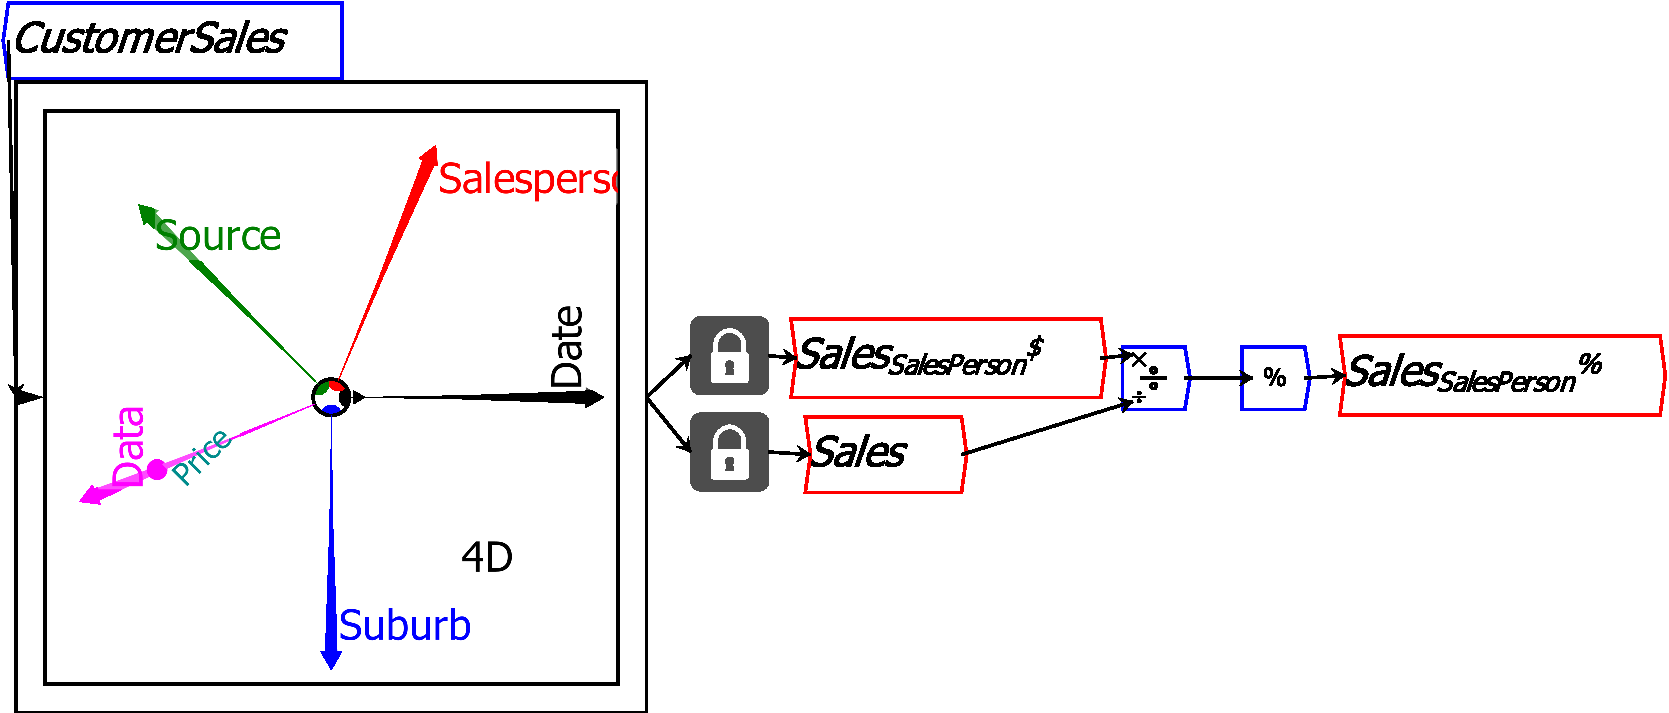
\includegraphics[width=\textwidth]{images/MergeExample01TwoVariables}

Sales\textsubscript{SalesPerson\textsuperscript{\$}and SalesPerson\textsuperscript{\%}}share
the same dimensions (SalesPerson and Date), and they can be separately
displayed as in the next figure.

\noindent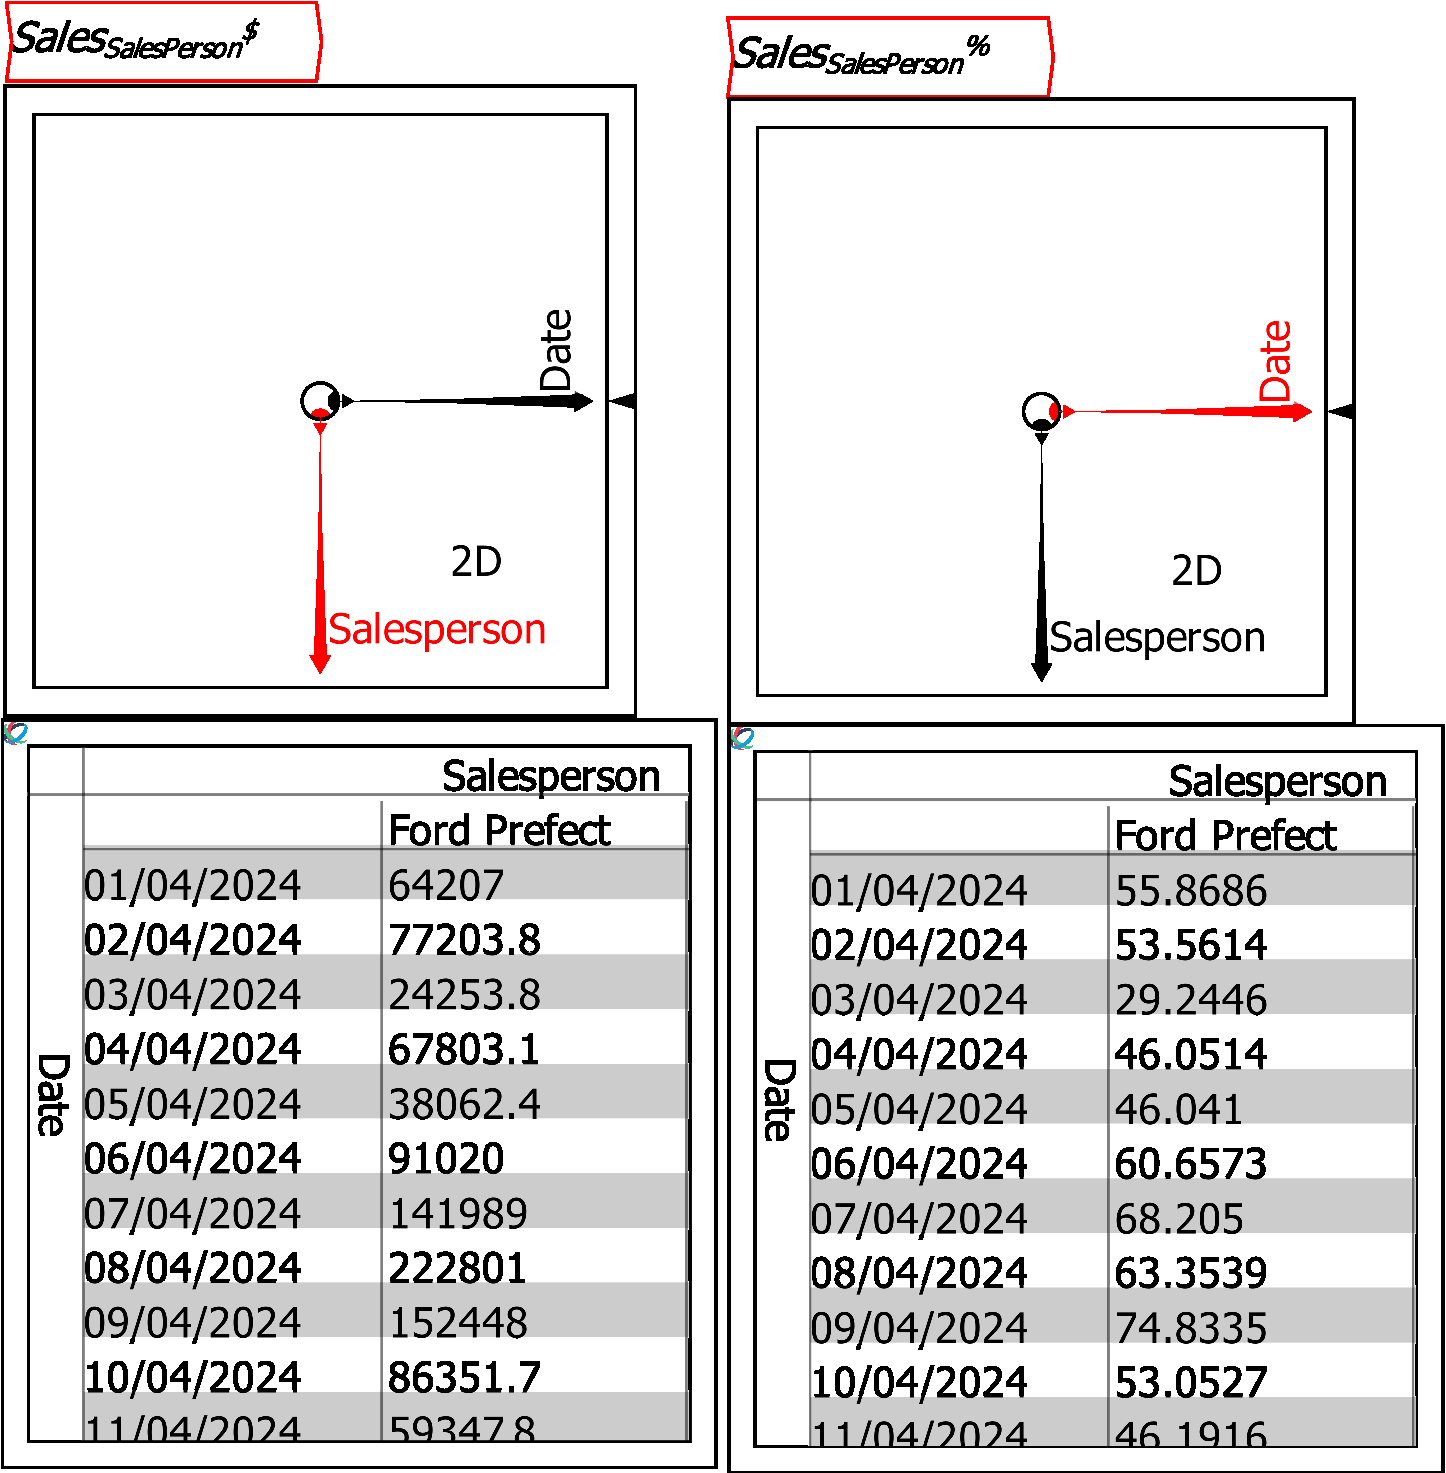
\includegraphics[width=\textwidth]{images/MergeExample02TwoVariablesSeparate}

Using the Merge operator, you can create one new Ravel containing
information from both the \$ sales and the \% of total sales analysis:

\noindent\includegraphics[width=\textwidth]{images/MergeExample02TwoVariablesEditForm}

The merged Ravel has 3 dimensions, with the extra dimension Analysis
now containing the Sales by dollar amount and Sales as a percentage
of total sales as entries on the Analysis axis.

\noindent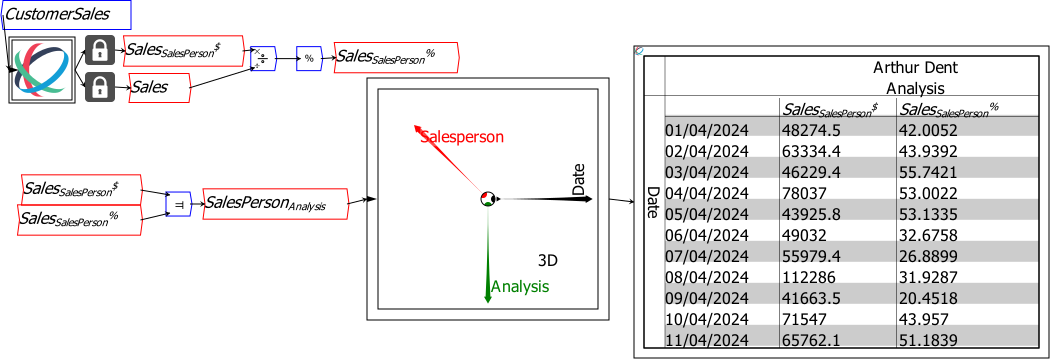
\includegraphics[width=\textwidth]{images/MergeExample03TwoVariablesMerged}

\subsubsection{Slice}

\label{Operation:slice}

\operatorKey{slice}

The operator can be placed on the canvas in two ways:
\begin{itemize}
\item From the \emph{Tensor Operations (``tensor'')} toolbar \buttonIcon{innerProduct};
or 
\item By typing the letters ``slice'' on the canvas and then pressing the
Enter key.
\end{itemize}
Slice will cut off a tensor along a given axis by the argument, as
configured in the operation edit dialog. For example $\mathrm{slice}(\{x_{1},x_{2},\ldots x_{n}\},3)=\{x_{1},x_{2},x_{3}\}$.
If the tensor is rank one (ie a vector), it is not necessary to specify
the axis.

If the slice argument is negative, then it refers to the number of
elements from the end of that axis. For example $\mathrm{slice}(\{x_{1},x_{2},\ldots x_{n}\},-3)=\{x_{n-2},x_{n-1},x_{n}\}$.

\subsubsection{Size}

\label{Operation:size}

\operatorKey{size}

The operator can be placed on the canvas in two ways:
\begin{itemize}
\item From the \emph{Tensor Operations (``tensor'')} toolbar \buttonIcon{innerProduct};
or 
\item By typing the letters ``size'' on the canvas and then pressing the
Enter key.
\end{itemize}
Size refers to the number of elements along a named dimension given
by the operation axisargument---eg a $3\times2$ rank 2 tensor with
named axes ``0'' and ``1'', size(``1'')==2.

If the axis argument is left blank, the size returns the total number
of elements present in the tensor. This may be less than the product
of axis sizes if the data is sparse---which will normally be the
case.

\subsubsection{Shape}

\label{Operation:shape}

\operatorKey{shape}

The operator can be placed on the canvas in two ways:
\begin{itemize}
\item From the \emph{Tensor Operations (``tensor'')} toolbar \buttonIcon{innerProduct};
or 
\item By typing the letters ``shape'' on the canvas and then pressing the
Enter key.
\end{itemize}
Returns a vector of axis sizes. Coupling this operation with a
\htmlref{gather}{Operation:gather} operation and variable would allow
you interactively select axis size.

\subsection{Statistical Operations}
\label{operations-statistics}

\subsubsection{Mean}

\label{Operation:mean}

\operatorKey{mean}

The operator can be placed on the canvas in two ways:
\begin{itemize}
\item From the \emph{Statistics (``statistics'')} toolbar \buttonIcon{mean};
or 
\item By typing the letters ``mean'' on the canvas and then pressing the
Enter key
\end{itemize}
Returns the mean (or average) along a named dimension of all elements
present. If the dimension is not named, then the mean is over all
elements present in the tensor. Note that missing elements are not
counted.

\subsubsection{Median}

\operatorKey{median}
\label{Operation:median}

The operator can be placed on the canvas in two ways:
\begin{itemize}
\item From the \emph{Statistics (``statistics'')} toolbar \buttonIcon{mean};
or 
\item By typing the letters ``median'' on the canvas and then pressing the
Enter key
\end{itemize}
Returns the median along a named dimension of all elements present.
If the dimension is not named, then the median is over all elements
present in the tensor.

\subsubsection{Standard Deviation}

\label{Operation:stdDev}

\operatorKey{stdDev}

The operator can be placed on the canvas in two ways:
\begin{itemize}
\item From the \emph{Statistics (``statistics'')} toolbar \buttonIcon{mean};
or 
\item By typing the letters ``stdDev'' on the canvas and then pressing the
Enter key
\end{itemize}
Returns the standard deviation along a named dimension of all elements
present. If the dimension is not named, then the standard deviation
is over all elements present in the tensor. Note that missing elements
are not counted.

\[
\sigma=\frac{1}{N-1}\sum_{i}^{N}(x_{i}-\langle x\rangle)^{2}
\]


\subsubsection{$k$-th moment}

\label{Operation:moment}

\operatorKey{moment}

The operator can be placed on the canvas in two ways:
\begin{itemize}
\item From the \emph{Statistics (``statistics'')} toolbar \buttonIcon{mean};
or 
\item By typing the letters ``moment'' on the canvas and then pressing the
Enter key
\end{itemize}
Returns the $k$-th moment about the mean along a named dimension
of all elements present. $k$ is specified by the numerical argument
of the operation, which defaults to 1 (hence the result will be 0
in that case). If the dimension is not named, then the $k$-th moment
is over all elements present in the tensor. Note that missing elements
are not counted.

\[
\langle\Delta x^{k}\rangle=\frac{1}{N}\sum_{i}(x_{i}-\langle x\rangle)^{k}
\]

Also 
\[
\sigma^{2}=\frac{N}{N-1}\langle\Delta x^{2}\rangle
\]


\subsubsection{Histogram}

\label{Operation:histogram}

\operatorKey{histogramKey}

The operator can be placed on the canvas in two ways:
\begin{itemize}
\item From the \emph{Statistics (``statistics'')} toolbar \buttonIcon{mean};
or 
\item By typing the letters ``histogram'' on the canvas and then pressing
the Enter key
\end{itemize}
Computes the histogram along a named dimension of all elements present.
If the dimension is not named, then the histogram is over all elements
present in the tensor. The number of bins is specified by the numeric
argument to the operation.
\begin{center}
\resizebox{\textwidth}{!}{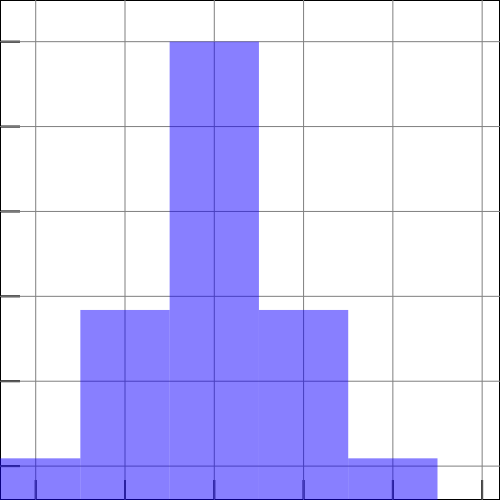
\includegraphics{images/histogram}}
\par\end{center}

\begin{center}
{\em An example usage of the histogram operation} 
\par\end{center}

\subsubsection{Covariance}

\label{Operation:covariance}

\operatorKey{covariance}

The operator can be placed on the canvas in two ways:
\begin{itemize}
\item From the \emph{Statistics (``statistics'')} toolbar \buttonIcon{mean};
or 
\item By typing the letters ``covariance'' on the canvas and then pressing
the Enter key
\end{itemize}

Computes the covariance of two tensors along named dimension. If the
inputs are of rank $N$ and $M$ respectively, the output will be
a $(N-1)\times(M-1)$ rank tensor, where the $(i,j)$ element is the
covariance of the $i$-th slice of the first argument along the named
dimension, and the $j$-th slice along the named dimension. As such,
it is conformant with the definition of \texttt{cov} function in Octave,
but not with the equivalently named function in Matlab: 
\begin{quote}
Compatibility Note:: Octave always treats rows of X and Y as multivariate
random variables. For two inputs, however, MATLAB treats X and Y as
two univariate distributions regardless of their shapes, and will
calculate covariance whenever the number of elements in X and Y are
equal. This will result in a 2x2 matrix. Code relying on MATLAB's
definition will need to be changed when running in Octave. 
\end{quote}
If only a single argument $x$ is supplied to the covariance, then
the result is equivalent to cov$(x,x)$, ie each slice is covaried
with each other slice.

The formula for covariance between stochastic variables $x$ and $y$
is 
\[
\mathrm{cov}(x,y)=\frac{1}{N-1}\sum_{i}(x_{i}-\langle x\rangle)(y_{i}-\langle y\rangle)
\]

\subsubsection{Correlation coefficient $\rho$}\label{Operation:correlation}

\label{Operation:rho}

\operatorKey{rhoCorrelationCoefficient}

The operator can be placed on the canvas in two ways:
\begin{itemize}
\item From the \emph{Statistics (``statistics'')} toolbar \buttonIcon{mean};
or 
\item By typing the letters ``correlation'' on the canvas and then pressing
the Enter key
\end{itemize}
See \htmlref{covariance}{Operation:covariance} for the interpretation of tensor valued
arguments. The correlation coefficient is defined as

\[
\rho(x,y)=\frac{\mathrm{cov(x,y)}}{\sigma(x)\sigma(y)}
\]

\subsubsection{Linear Regression}\label{Operation:linearRegression}

This operation performs linear regression of the inputs along a named
dimension. The output has the same rank and x-vector as the $x$ input,
and consists of the linear fitted $y$ values.

The slope and intercept of the fitted line is available as a tooltip.

\noindent
\includegraphics[width=\textwidth]{images/linearRegression}

\subsection{Switch}

\label{SwitchIcon}

\operatorKey{switchKey}

The operator can be placed on the canvas by clicking on its icon \buttonIcon{switch}on
the widget bar.

A switch block (also known as a case block, or select in the Fortran
world) is a way of selecting from a range of alternatives according
to the value of the input, effectively defining a piecewise function.
\begin{center}
\resizebox{\textwidth}{!}{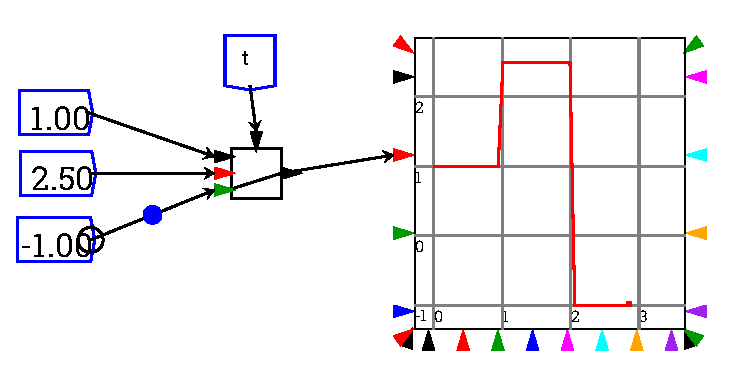
\includegraphics{images/switch}} {\em
An example switch block with 3 cases} 
\par\end{center}

The default switch has two cases, and can be used to implement an
if/then/else construct. However, because the two cases are 0 and 1,
or false and true, a two case switch statement will naturally appear
``upside down'' to how you might think of an if statement. In other
words, it looks like:

\noindent\parbox[c]{1\textwidth}{%
 \texttt{if not }{\em condition} \texttt{then}\\
 \ldots\texttt{else}\\
 \ldots %
}

You can add or remove cases through the context menu.

\subsection{User defined function}

\label{Operation:userFunction}\label{UserFunction}

\operatorKey{userFunction}

A user defined function is a functioned defined by an algebraic expression.
Support for this feature is courtesy of the wonderful \htmladdnormallink{exprtk}{http://www.partow.net/programming/exprtk/index.html}
library developed by Arash Partow.

A user defined function has a {\em name}, {\em parameters} and
an {\em expression}. Example expressions are things like \verb'x+y'
or \verb'sin(x)'. More details of the sorts of expressions possible
can be found in the \htmlref{User Defined Functions}{ExprTk}
section of the manual.

The parameters are specified as part of the name, so a user defined
function adding x and y would be called \verb'useradd(a,y)' and the
sin example might be called \verb'mysin(x)'. Functions with up to
two arguments can be wired on the canvas. User defined functions can
call other user defined functions, so specifiying more than 2 parameters
can be a useful thing to do.

\subsection{Godley Tables}

\label{godley}\label{GodleyIcon}

A Godley Table employs double-entry bookkeeping to create dynamic
models of monetary transactions. It can also be used to build dynamic
models of systems based on transitions between exclusive categories---such
as epidemiological systems like SEIRD models of disease transmission.

A Godley Table uses the rules of accounting to create consistent equations
to describe financial flows. The essential rules are that:
\begin{itemize}
\item Each flow must be entered twice on its row; and
\item The sum of $Assets-Liabilities-Equity$ must equal zero on each row.
\end{itemize}
Using these rules, \emph{Minsky} develops stock-flow consistent models
of financial transactions. The row entries are flows in differential
equations for the stocks. For example, the Godley Table shown in the
next figure:

\noindent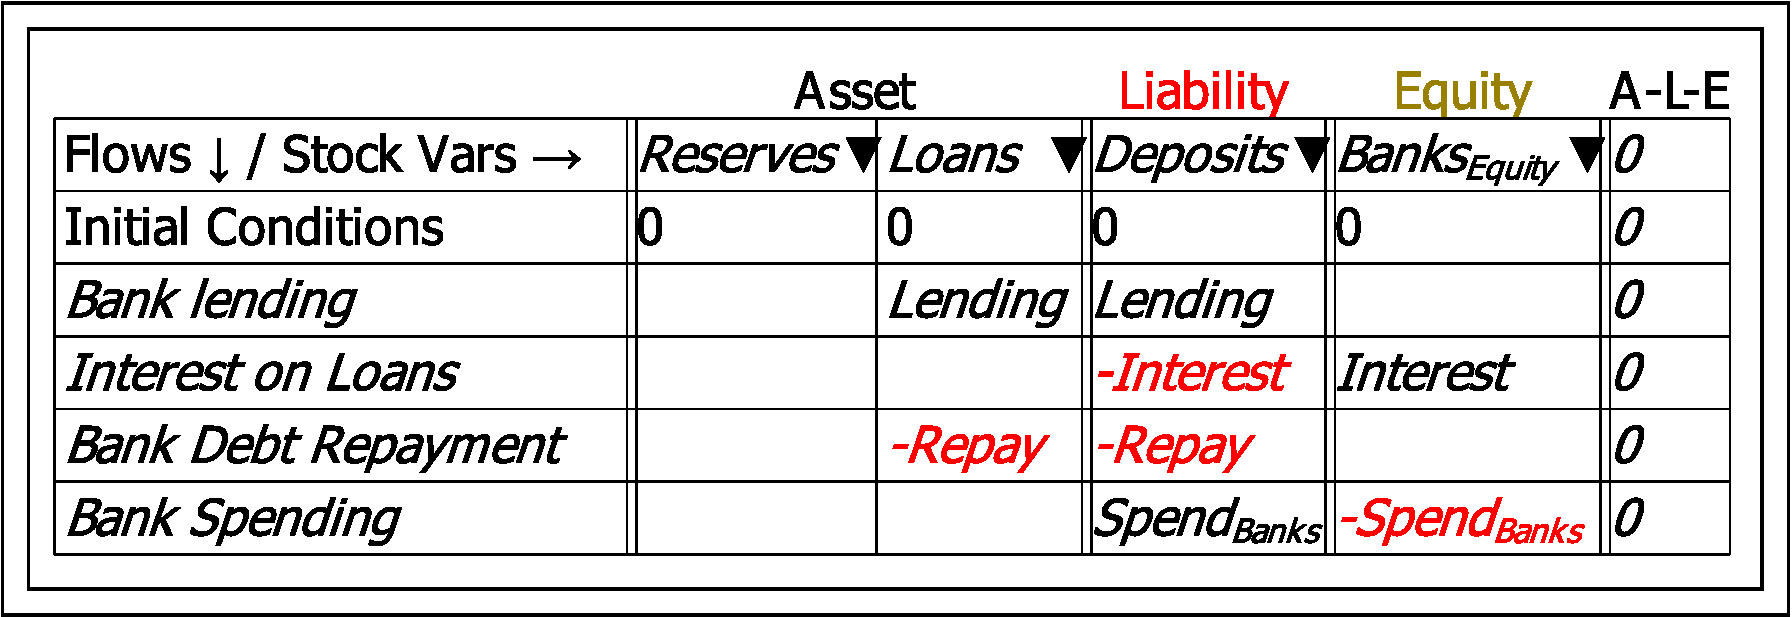
\includegraphics[width=\textwidth]{images/GodleyTableImages}

generates the following set of differential equations:

$\begin{array}{c}
\frac{d}{dt}Loans=Lending-Repay\\
\frac{d}{dt}Deposits=Lending-Interest-Repay+Spend_{Banks}\\
\frac{d}{dt}Banks_{Equity}=Interest-Spend_{Banks}\\
\frac{d}{dt}Reserves=0
\end{array}$

Stocks are thus completely defined by the Godley Table itself as equations
in a set of coupled differential equations. For this reason, when
placed on the canvas, each stock has an output but no input. Flows,
on the other hand, have both inputs and outputs, and have to be fully
defined on the canvas itself.

For complete details see \htmlref{Godley tables}{Godley-Tables}.

\subsubsection{Creating a Godley Table}

To insert a Godley Table into a model, click on the Godley icon \buttonIcon{GodleyIcon}on
the Operations bar. This attaches a Godley Table to your cursor. Click
where you wish to place it on the canvas and this object will be inserted:

\noindent
\includegraphics[width=\textwidth]{images/GodleyTableIconMode}

You can edit this object by either double-clicking on the icon, or
by choosing ``Edit Godley Table'' from its context menu.

\subsubsection{Godley Table Context Menu}

The Godley-Table-specific commands in the context menu are:

\begin{tabular}{|c|p{0.65\textwidth}|}
\hline 
Command & Effect\tabularnewline
\hline 
\hline 
Open Godley Table & Opens the form for editing Godley Tables\tabularnewline
\hline 
Title & Give the Table a name which is displayed on the icon and edit form\tabularnewline
\hline 
Set currency & If multiple currencies are used in a model, specify the currency for
the current table\tabularnewline
\hline 
Editor Mode & Convert the canvas view of the table from an icon to the table itself,
which can be edited on the canvas\tabularnewline
\hline 
Row/Col buttons & When Editor Mode is active, show row and column buttons used to add
and delete rows and columns\tabularnewline
\hline 
Display Variables & Show the stocks and flows defined in the table as variables attached
to the table in icon view\tabularnewline
\hline 
Copy flow variables & Copy all the flow variables in the table to the canvas\tabularnewline
\hline 
Copy stock variables & Copy all the stock variables in the table to the canvas\tabularnewline
\hline 
Export as & Export the table in either CSV or LaTeX format\tabularnewline
\hline 
Rotate GodleyIcon & This command has been deprecated and will be deleted in a future release\tabularnewline
\hline 
\end{tabular}

\subsubsection{Open Godley Table}

This commands bring up a dedicated window for editing a Godley Table:

\noindent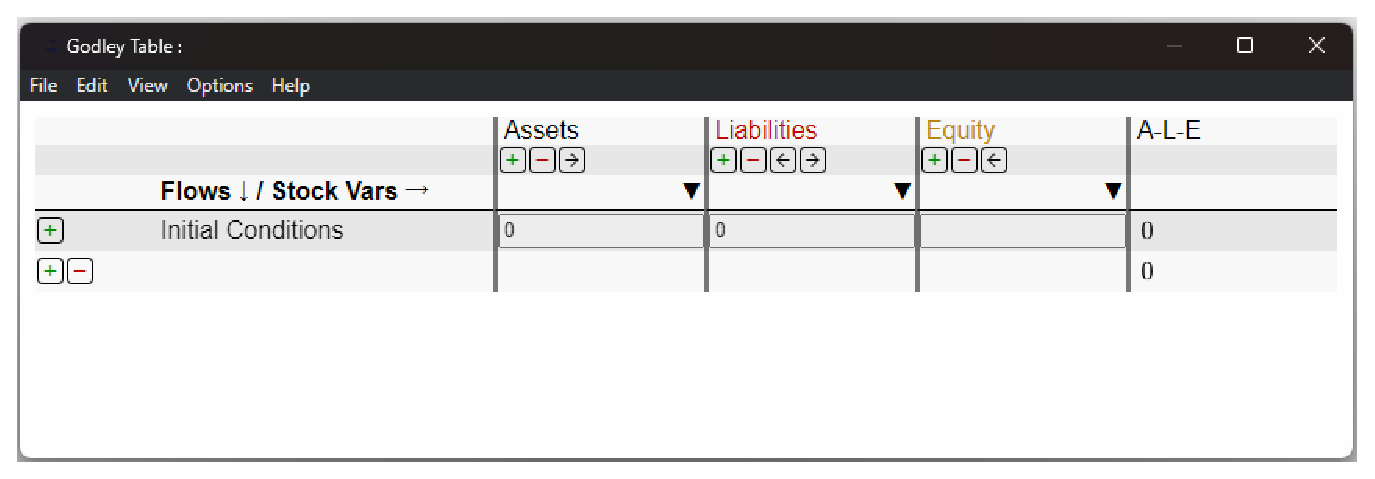
\includegraphics[width=\textwidth]{images/GodleyTableEditWindow}

\paragraph{Defining Stocks and Flows}

A Stock is defined by entering its name in the row on which the label
\emph{Flows\textdownarrow /Stock Vars\textrightarrow{}} is shown.
Normally these stocks will be bank accounts, though Godley Tables
can be used to model any dynamic system in which the stocks define
exclusive categories---such as a epidemiological model of disease
transmission, in which the population is divided into mutually exclusive
categories such as Infected or Uninfected, in Hospital or Not in Hospital,
etc.

Stocks are classified as either \emph{Assets}, \emph{Liabilities }or
\emph{Equity}, and the default form enables the entry of only one
Asset, Liability and Equity (similarly, there is only one row for
recording flows on the default form). To add more columns for accounts,
click on the + key below the relevant class (similarly, additional
rows for financial transactions are added by clicking on the + key
next to a row). This creates an additional column for entering stock
names. The - key deletes a stock, and the arrow keys move stocks right
and left as desired. 

If you press the leftarrow key on the first entry in Liabilities,
\emph{Minsky} will warn you that this will change the classification
of the stock from a Liability to an Asset.

The final column in the Table, labelled $A-L-E$, checks whether the
row sums to zero---which it must do to obey the rules of accounting.
The entries in the columns, and the sum itself, are \emph{symbolic}:
words are entered rather than numbers. The sum of that row must be
zero according to this formula. Normally this will involve two entries
of the same word---for example, \emph{Lending}---though fractional
entries are possible: $Lending-0.7Lending-0.3Lending$ still sums
to zero.

Three stocks and flows have been defined in the following figure. 

\noindent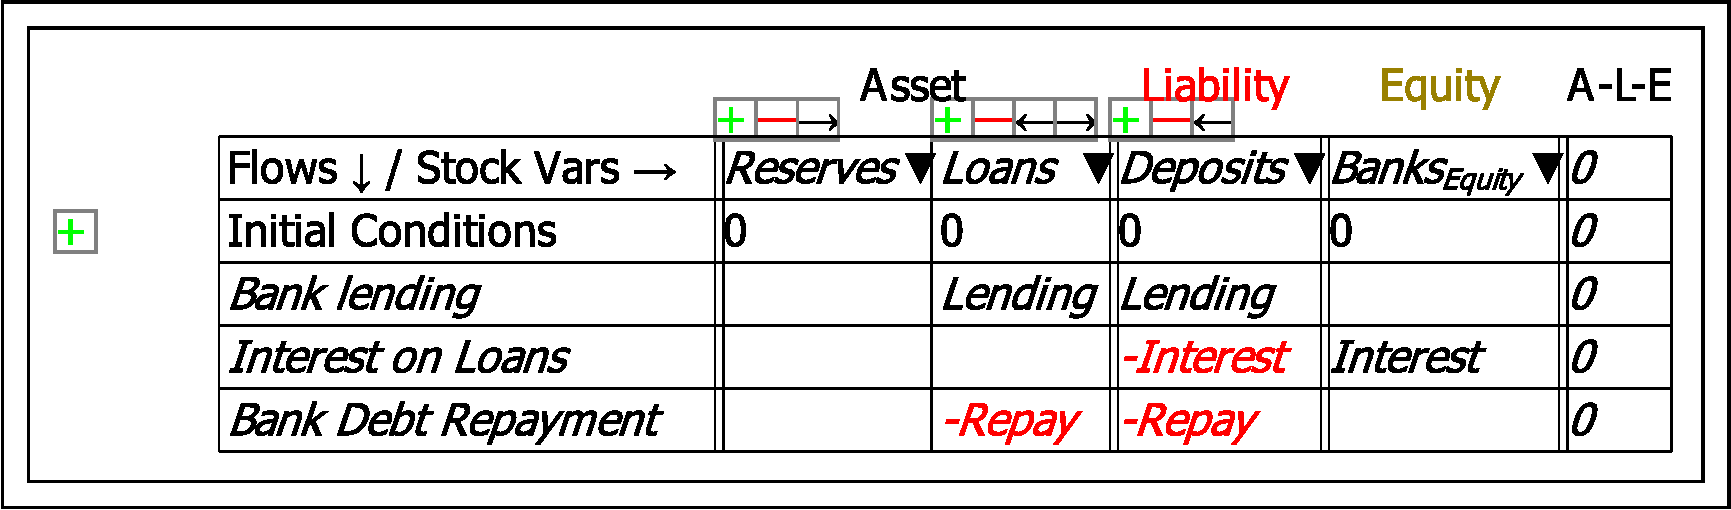
\includegraphics[width=\textwidth]{images/GodleyTableEditMode3StocksAndFlows}

\paragraph{Initial Conditions}

These are the values which the stocks take at the beginning of a simulation.
This row must also sum to zero, to ensure stock-flow consistency.

\subsubsection{Editor Mode}

This toggle command converts the canvas display of the Godley table
from the icon to a double-entry bookkeeping view:

\noindent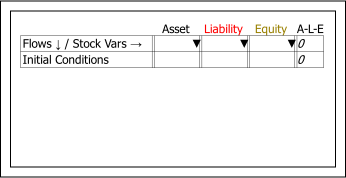
\includegraphics[width=\textwidth]{images/GodleyTableEditMode}

\subsubsection{Row/Col buttons}

This toggle command adds row and column buttons to a double-entry
bookkeeping view of the table on the canvas, so that it can be edited
on the canvas as an alternative to editing in the dedicated window.

\noindent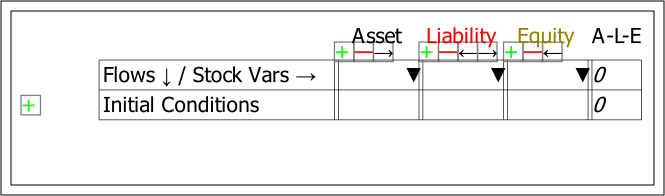
\includegraphics[width=\textwidth]{images/GodleyTableEditModeButtons}

\subsubsection{Display Variables}

This toggle command places the stocks (bank accounts) and flows (financial
transactions) entered in a Godley Table as variables on the Design
canvas, attached to the Godley Table icon itself.

\noindent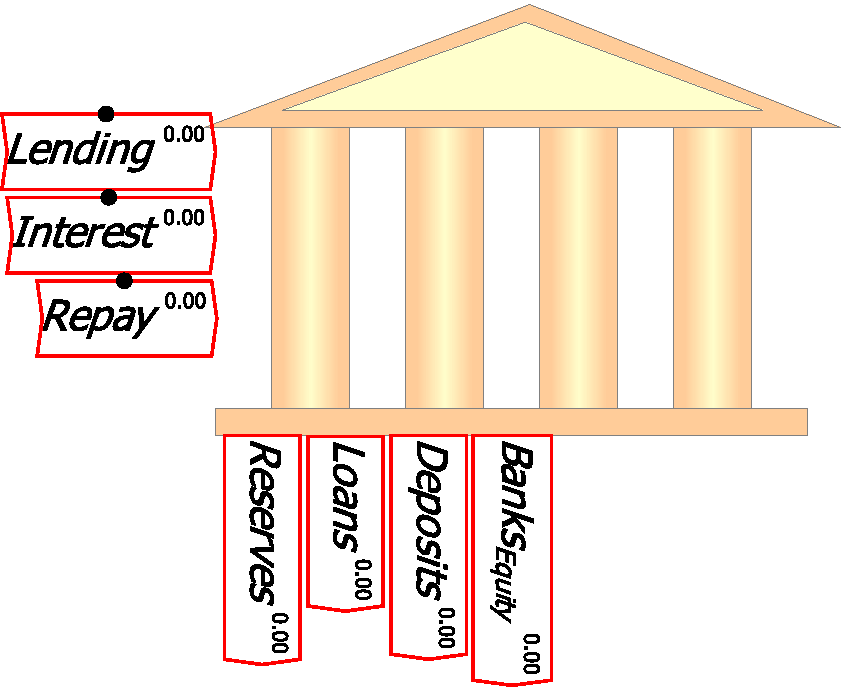
\includegraphics[width=\textwidth]{images/GodleyTableIconModeShowVariables}

\subsubsection{Copy Stock/Flow Variables}

These commands copy all Stocks or all Flows from a Godley Table and
attach them to the mouse cursor, for placement on the canvas. The
flows can then be defined using \emph{Minsky}'s mathematical operators
(Stocks are already completely defined by the Godley Table itself).
The next figure shows the result of using both these commands to place
all stocks and flows on the canvas.

\noindent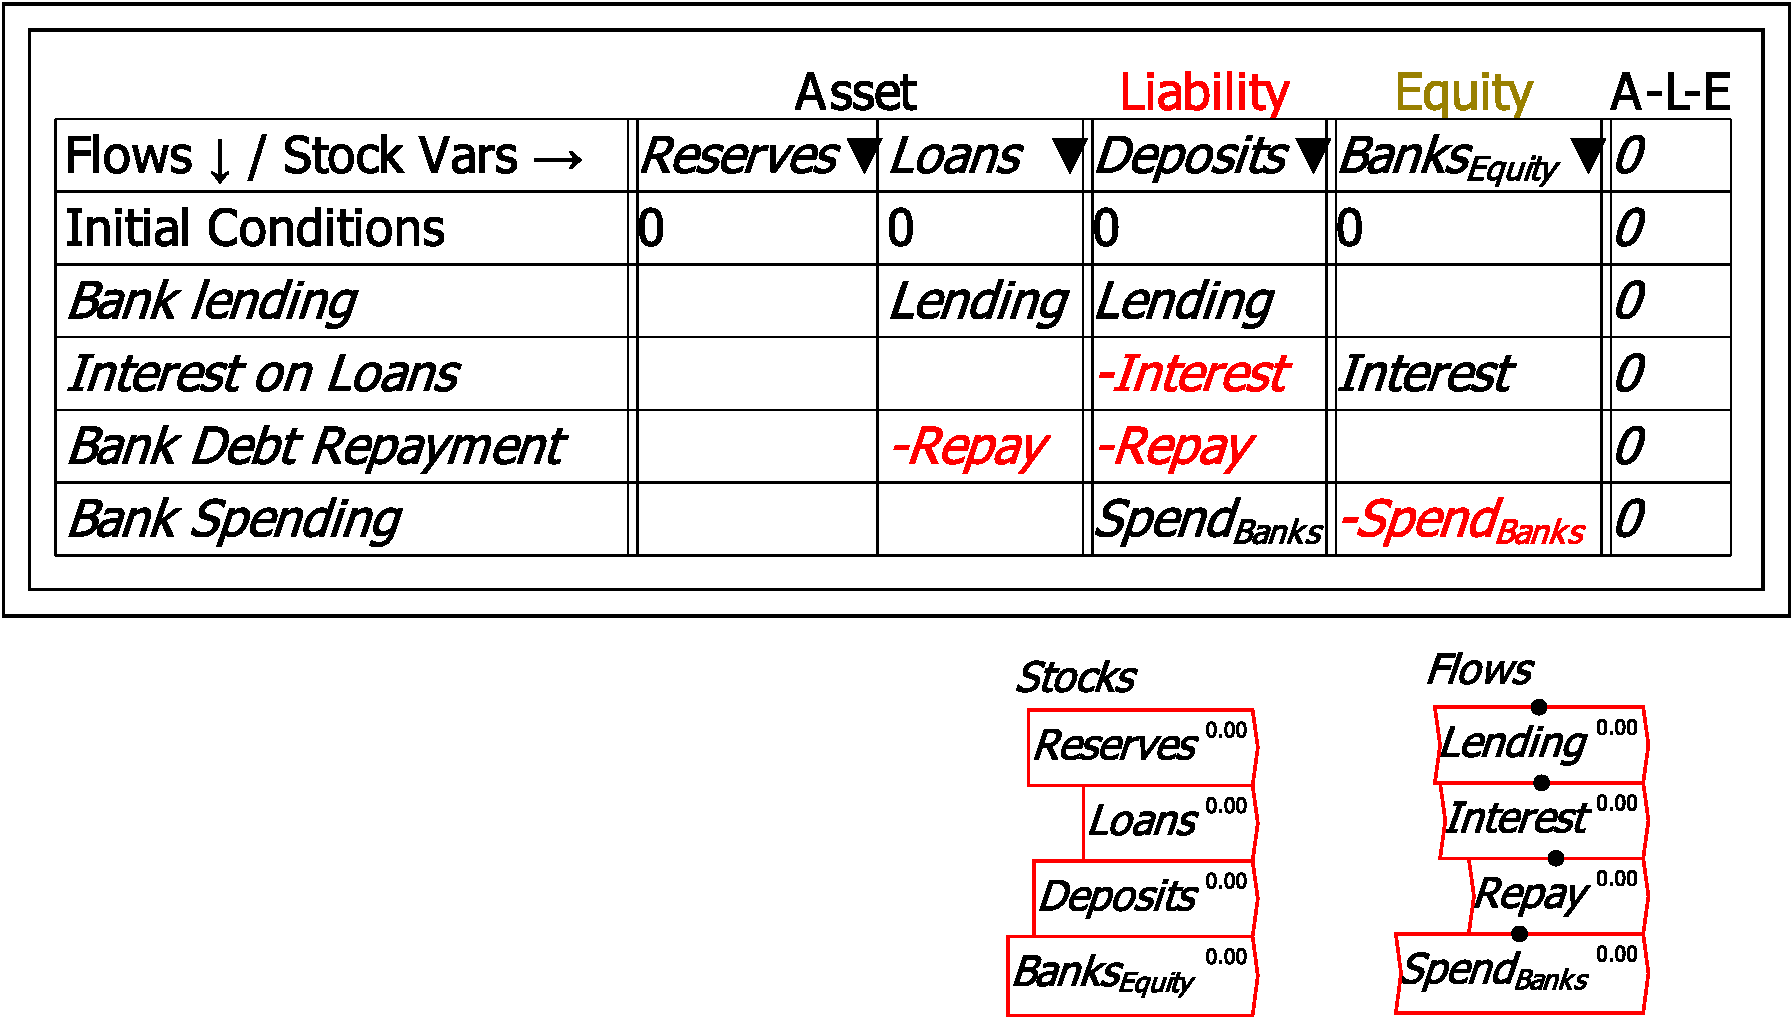
\includegraphics[width=\textwidth]{images/GodleyTableImagesStocksFlowsOnCanvas}

\subsubsection{Create multiple related Godley Tables}

\emph{Minsky} uses the fact that one entity's financial asset is another's
financial liability to rapidly build interlocked Godley Tables, which
describe the financial system from the perspective of every entity
or sector modelled in it. The inverted wedge \textifsymbol[ifgeo]{99}
next to the name of every column is used to check for Assets that
have not yet been recorded as a Liability, and vice versa. The next
figure shows an expanded Godley Table for the Banking Sector, with
additional Tables added for the Non-bank private sector, the Central
Bank, and the Treasury.

\noindent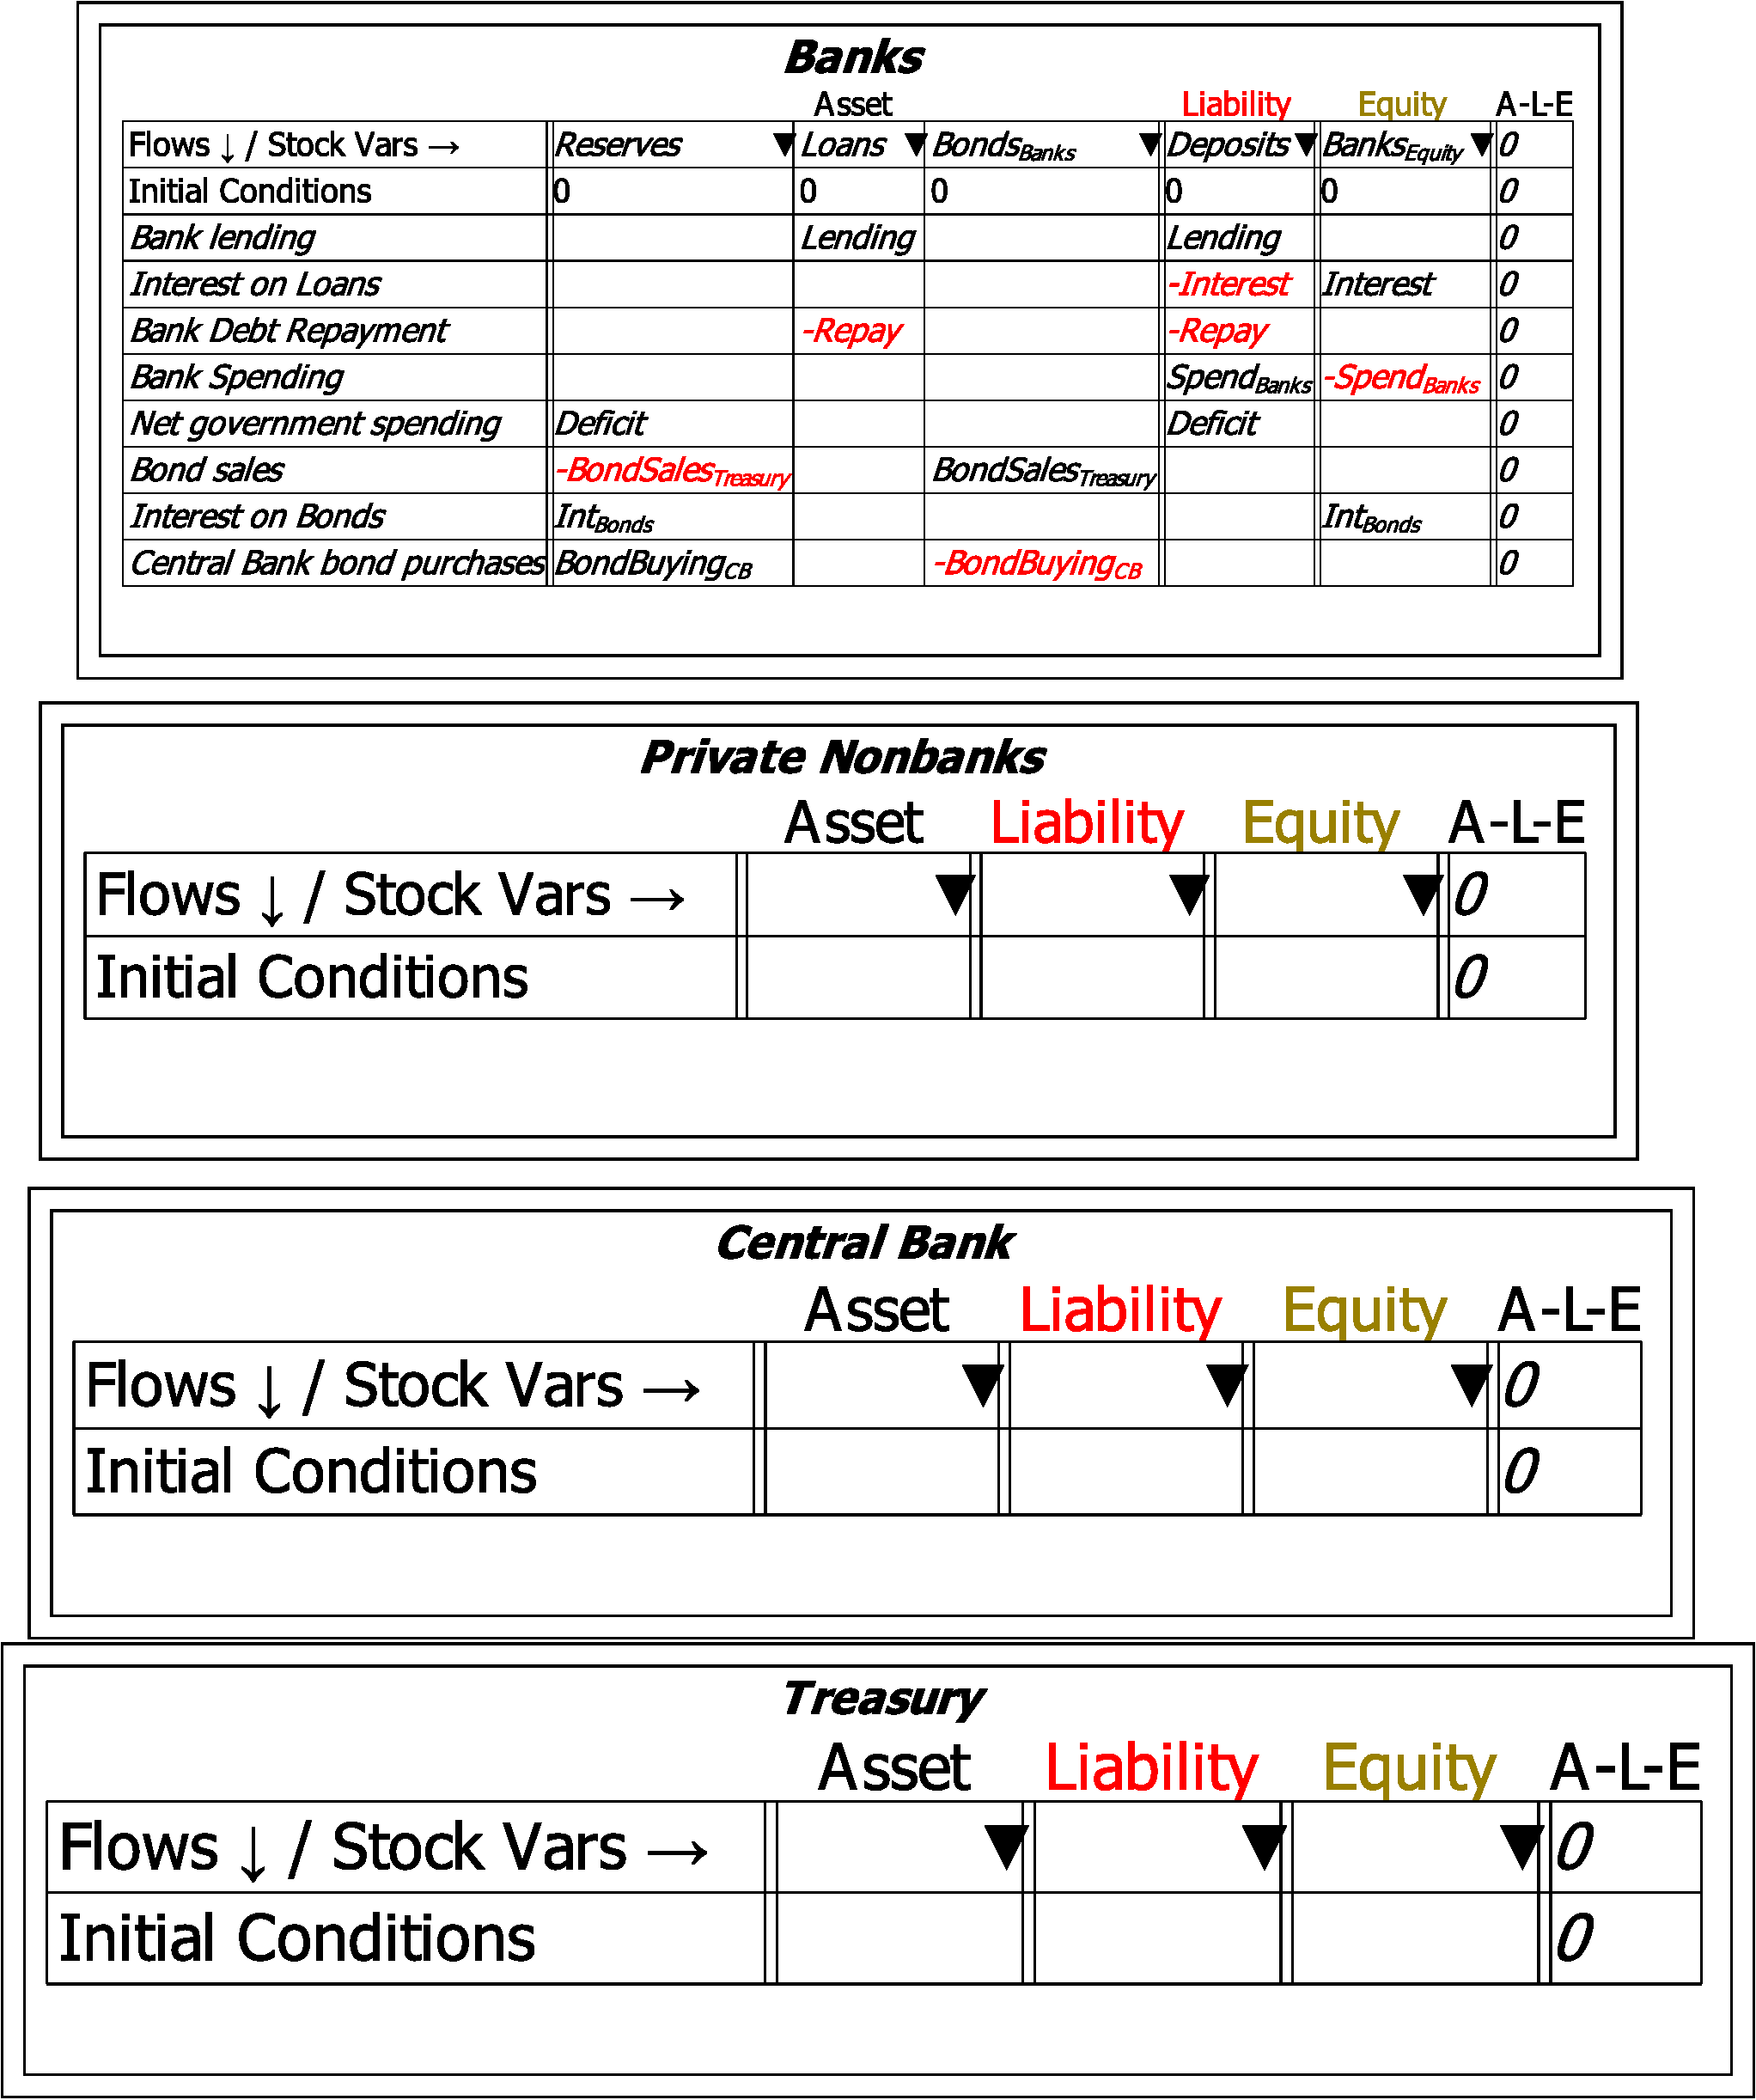
\includegraphics[width=\textwidth]{images/GodleyTableImagesMultiTablesUnfinished}

As well as auto-completing much of the additional Godley Tables, the
system indicates the need for additional accounts that are not part
of the initial Banks Godley Table. Central Bank purchases of bonds
from private banks indicate the need for the \emph{Asset Bonds}\textsubscript{\emph{CB}},
while the deficit indicates the need to add the Treasury's account
at the Central Bank, the ``Consolidated Revenue Fund'', as an additional
liability of the Central Bank.

\noindent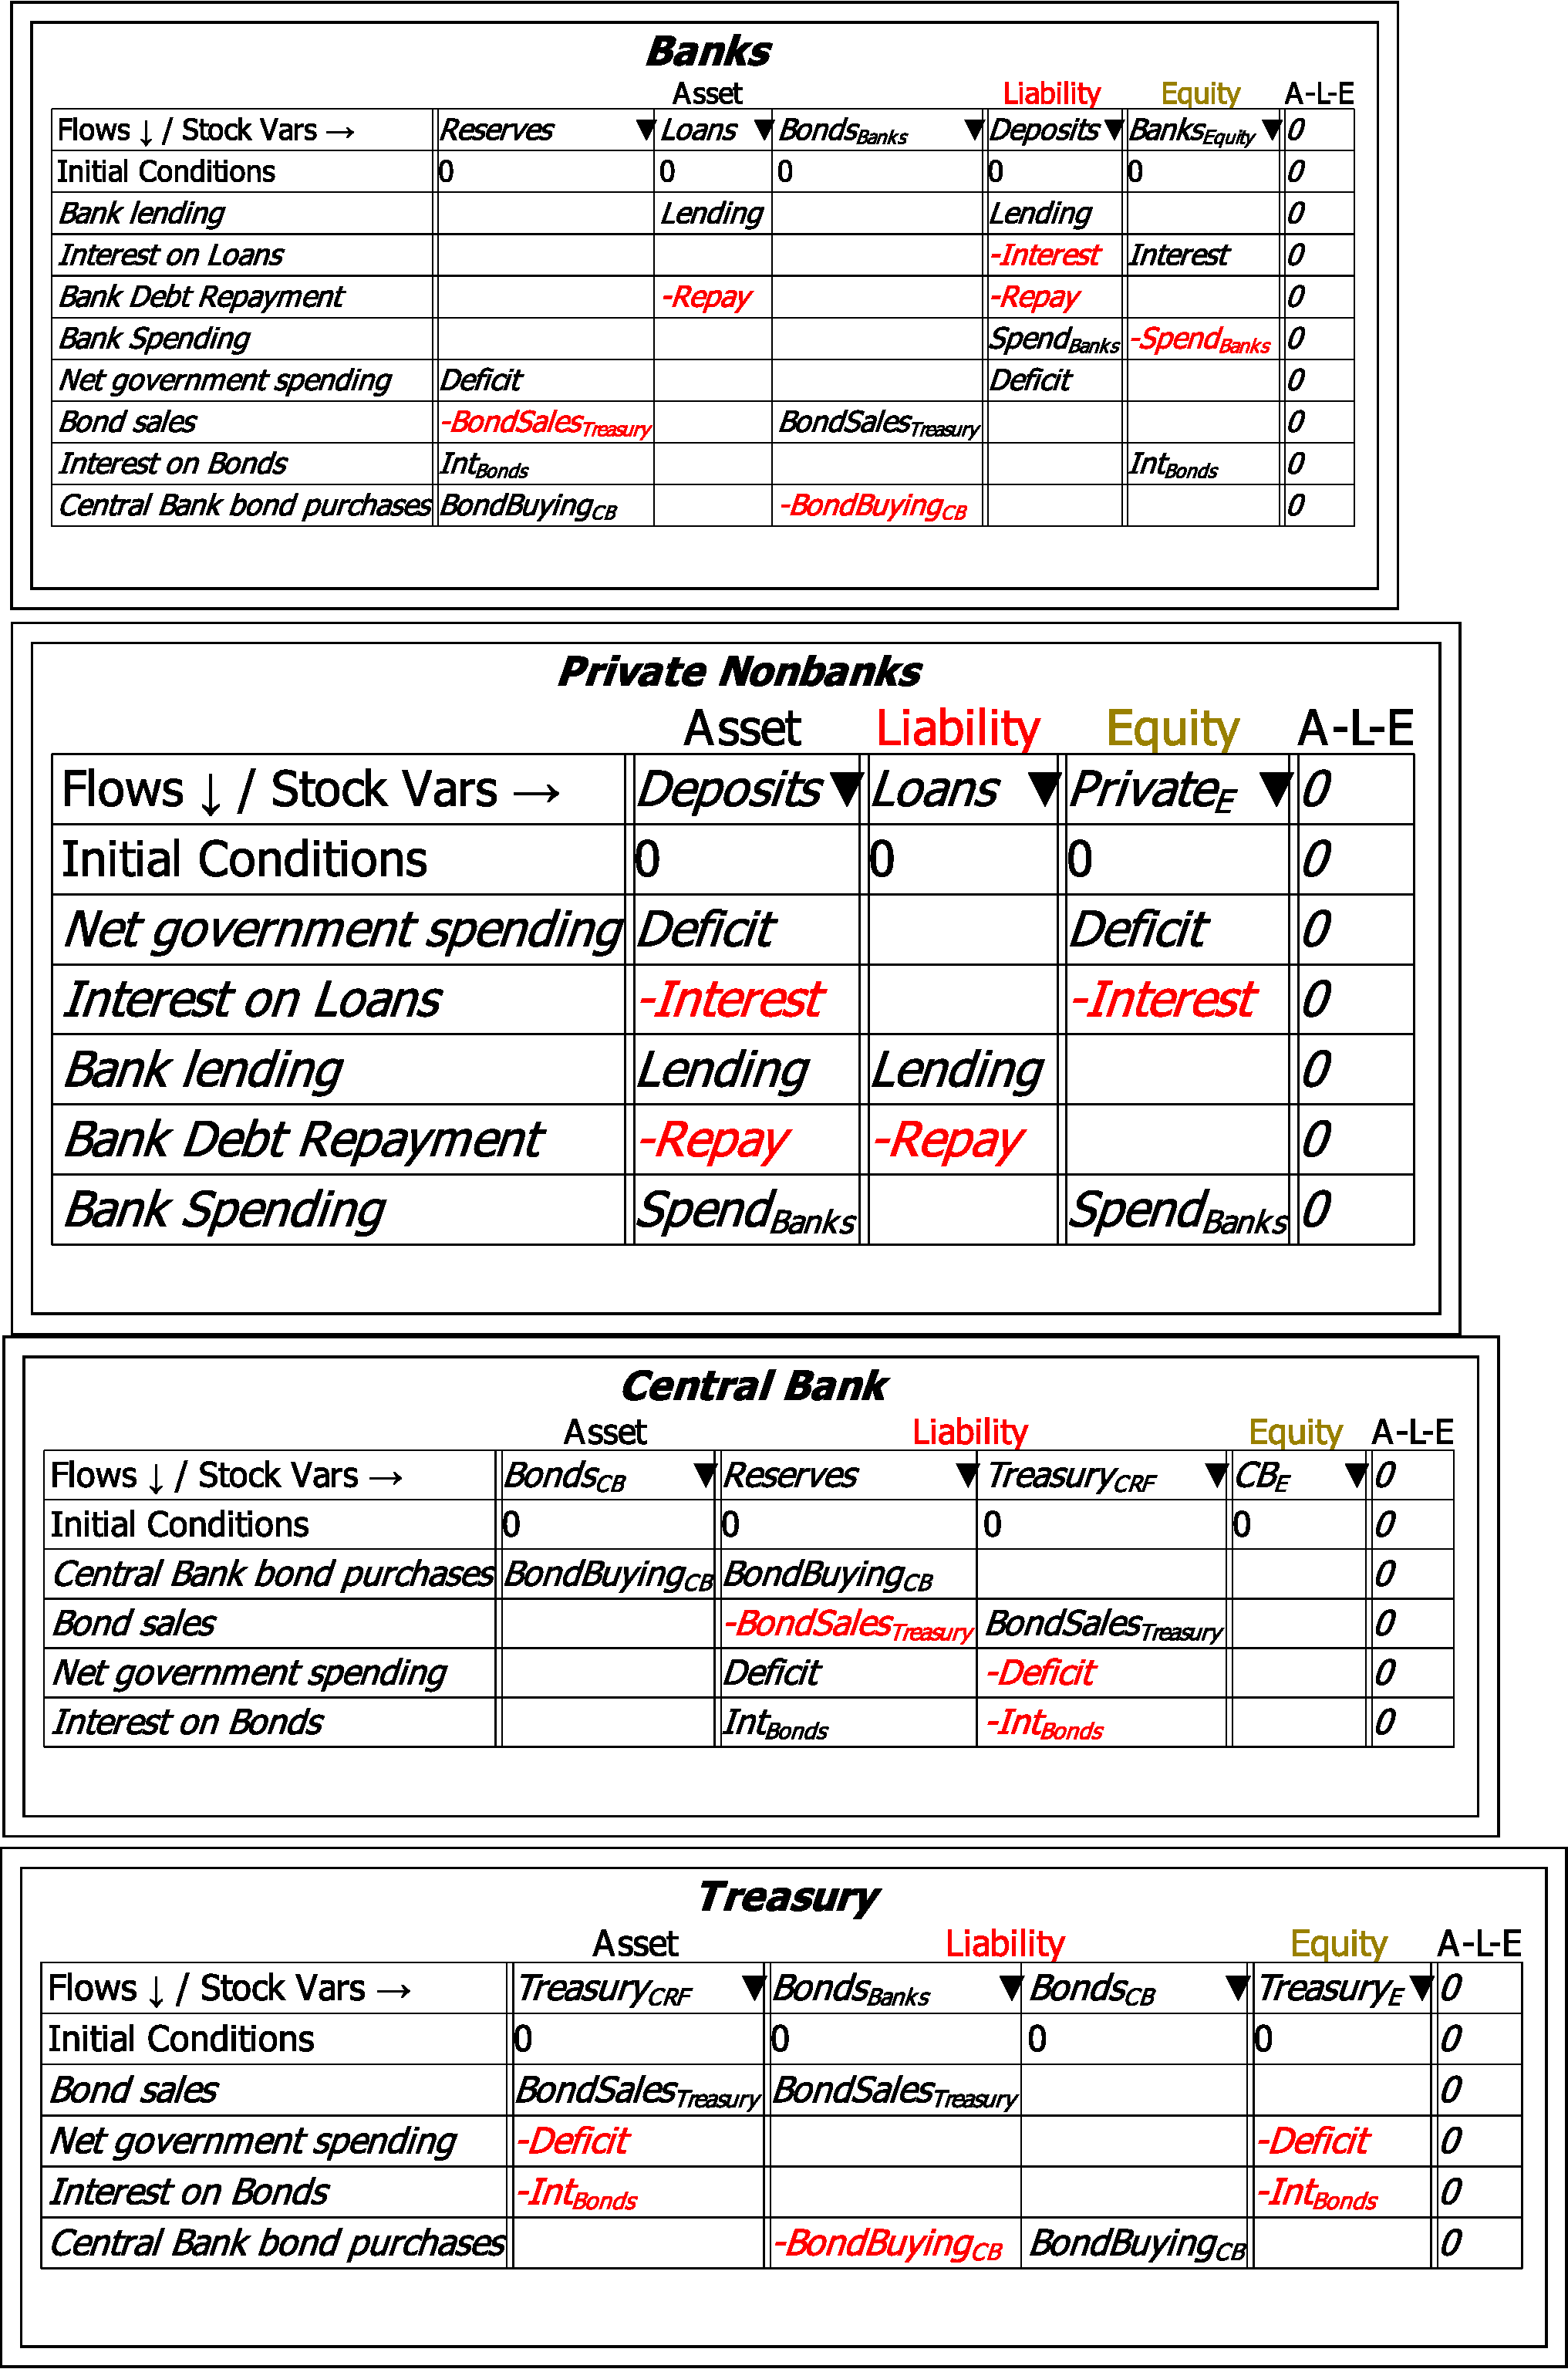
\includegraphics[width=\textwidth]{images/GodleyTableImagesMultiTablesFinished}

The inverted wedge next to the Equity column supports \emph{nonfinancial
}assets---things like houses, and shares valued in excess of their
limited liability. If these are included amongst the assets of an
entity, then they can also be recorded as an Equity of that entity
(this feature is still under development).

\subsubsection{Godley Table Context Menu}

The Godley Table Form has a context menu which assists in the rapid
completion of a multi-Godley-Table model. Entries can be copied from
one cell and pasted into another, and Flows in the model can be inserted
into a Godley Table cell as a positive or a negative entry:

\noindent\includegraphics[width=\textwidth]{images/GodleyTableContextMenu}

It is also possible to record all as-yet-unclassified flows as additions
to or substractions from the Equity of the relevant sector---which
is often (but not always) what is needed to complete a set of interlocking
Godley Tables. In the figure above, $-Interest$ and $+Spend_{Banks}$
are shown in the $A-L-E$ checksum column. Choosing ``Balance equity''
from the context menu transfers both these entries to the Equity column.

\subsubsection{Export Godley Table}

This command exports the Godley Table either as a CSV file, or a LaTeX
file, which can be imported into other programs for documentation
purposes.

\subsection{integrate $\int dt$}

\label{IntOp} Creates an integration (or stock) variable.

\operatorKey{integrate}

The operator can be placed on the canvas in two ways:
\begin{itemize}
\item From the integrate widget \buttonIcon{integrate} on the
toolbar; or 
\item By typing the letters ``integrate'' on the canvas and then pressing
the Enter key.
\end{itemize}
Integral blocks require two inputs: the flow being integrated, which
is attached to the top input on the block, labelled $f$; and the
initial conditions for the integral, which is attached to the bottom
input, labelled $0$.

\subsubsection{Integral Block context menu}

The integral-block-specific commands on the context menu are:

\noindent\begin{tabular}{|c|p{0.68\textwidth}|}
\hline 
Command & Effect\tabularnewline
\hline 
\hline 
Edit & Bring up the Edit form for this integrals\tabularnewline
\hline 
Copy item & Copy the variable name, rather than the combined integral block plus
name\tabularnewline
\hline 
Toggle var binding & Enable the integral block to be separated from the variable name\tabularnewline
\hline 
Rotate IntOp & Rotate the combined integral block plus name\tabularnewline
\hline 
\end{tabular}

Editable attributes include the variable's name and its initial value
at $t=0$. The main role of the Edit form is to provide the name for
the integrated variable---other details included on the form can
be controlled from elsewhere in the program. Type the name you want
to give the variable into the Name field and press Enter or click
on OK. You can also name the variable via the context menu item ``Rename
all instances''.

The flows to be integrated are connected to the top port of the integral
block, labelled `$f$'. The bottom port, labelled `0', can optionally
be connected to a constant, parameter or variable, which is used to
specify the initial value of the integral, following the same rules as
the \htmlref{variable initial value field}{var:init}.

\subsection{differentiate $d/dt$}

\operatorKey{differential}

\label{Operation:differentiate} Symbolically differentiates its input
with respect to system time, producing d/dt{[}input{]}. For further
explanation regarding differentiation, see \href{https://en.wikipedia.org/wiki/Derivative}{this wikipedia page}.


\section{Variables and Parameters}

\label{Variables}\label{Variable:constant}\label{VarConstant}\label{Variable:parameter}
\label{Variable:flow}\label{Variable:integral}\label{Variable:stock}

\operatorKey{var}

Variables represent values in a calculation, and come in a number
of varieties: 
\begin{description}
\item [{Constants}] represent an explicit numerical value, and do not have
a name. Their graphical representation shows the actual value of the
constant. 
\item [{Parameters}] are named constants. All instances of a given name
represent the same value, as with all other named variables, so changing
the value of one parameter, either through its edit menu, or through
a slider, will affect all the others of that name.

Parameters are used to import data from a \htmlref{CSV file}{CSV import},
which is how external data is imported into Ravel for analysis.

Parameters can also be used to generate arrays of numbers for
use in a \emph{Ravel} file using built-in formulas which are placed
in the ``Initial value'' field of the parameter definition form.
See \htmlref{tensor valued initial conditions}{tensor-init}.
\item [{Flow variables}] have an input port that defines how the value
is to be calculated. Only one flow variable of a given name can have
its input port connected, as they all refer to the same quantity.
If no input ports are connected, then flow variables act just like
parameters. 
\item [{Integral variables}] represent the result of integrating its input
over time by means of the differential equation solver. The integrand
is represented by the input to an integral operator that is attached
to the integral variable. 
\item [{Stock variables}] are the columns of Godley tables, and represent
the integral over time of the sum of the flow variables making up
the column. 
\end{description}
Variables may be converted between types in the variable edit menu,
available from the context menu, subject to certain rules. For example,
a variable whose input is wired anywhere on the canvas cannot be changed
from ``flow''. Stock variables need to be defined in a Godley table,
and so on.

\subsection{Variable names}

Variable names uniquely identify variables. Multiple icons on the
canvas with the same name at the same level all refer to the same
variable. Variable names can have local scope\index{local scope}, in which case it
is specific to the \htmlref{group}{Group} in which it is contained,
othewise its scope is determined by the innermost containing group
that has a local variable of that name. If no such variable exists,
its scope is global.

A variable which is local to a group can be used as a formula in
several locations in a file. For example, if you use a, b anc c as
constants in a polynomial $a+bx+cx^{2}$ and make them local to a
group, then the group can be used in several parts of a document, with
the argument x and the values of a,b and c being different in every
instance.

\subsection{Initial conditions}

\label{var:init}\index{initial conditions}

Variable initial conditions can be defined through the ``init value''
field of the variable edit menu, or in the case of Godley table stock
variables, through the initial condition row of the Godley table.
An initial value can be a simple number, or it can be a multiple of
another named parameter. In case of symbolic definitions, it would
be possible to set up a circular reference where the initial value
of variable A is defined in terms of the initial value of variable
B, which in turn depends on the intial value of A. Such a pathological
situation is detected when the system is reset.

\subsection{Tensor valued initial conditions}

\label{tensor-init}\index{initial conditions|tensor}

\emph{Ravel} provides a simple functional language which allows for
the generation of tensor-valued operations. This enables \emph{Ravel}
to work with hypothetical as well as actual data---for example, hypothetical
sales volumes for a new product from zero to 500,000 sales per year
can be generated using the iota formula by putting the expression
``iota(500001)'' in the initial value field for the variable \emph{Sales}.
This generates an axis/dimension named 0 with values from 0 to 500,000. 

These functions take the form {\em func}$(n_{1},n_{2},\ldots,n_{r})$
where $r$ is the desired rank, and $n_{1},n_{2},$ etc are the dimensions
of the tensor. Available functions include:

\begin{tabular}{|r|l|}
\hline 
name  & description\tabularnewline
\hline 
\verb+one+ & the tensor is filled with `1'\tabularnewline
\verb+zero+ & the tensor is filled with `0'\tabularnewline
\verb+iota+ & the arithmetic sequence $(0,1,...\prod_{i}n_{i})$\tabularnewline
\verb+eye+ & diagonal elements filled with `1', offdiagonal `0'\tabularnewline
\verb+rand+ & tensor filled with random numbers in the range $[0,1)$\tabularnewline
\hline 
\end{tabular}\index{one}\index{zero}\index{iota}\index{eye}\index{rand}
\begin{itemize}
\item \verb+eye+ is equivalent to \verb+one+ for vectors. 
\item \verb+rand+ generates different random numbers each time the simulation
is reset, and uses the clib \verb+rand()+ function. 
\end{itemize}

\subsection{Sliders}

Variables have a ``slider'' feature, which allows the value of the
variable (or parameter or constant) to be altered by the user via
the mouse or by arrowkeys.

The options Max, Min and Step Size in the Edit form let you control
the maximum and minimum values for the variable/parameter, and how
much the value changes for each press of an arrowkey. A relative slider
means that the step size is expressed as a fraction of max-min.

Adjusting the slider of an integral (or stock) variable while the
system is running actually adjusts the present value of the variable.
The sliders can also be adjusted using the keyboard arrow keys: uparrow
\textuparrow{} or rightarrow \textrightarrow{} increases the value
of the parameter by the step size; downarrow \textdownarrow or leftarrow
\textleftarrow{} reduces it.

\subsection{Variable Browser}

\label{VariableBrowser}

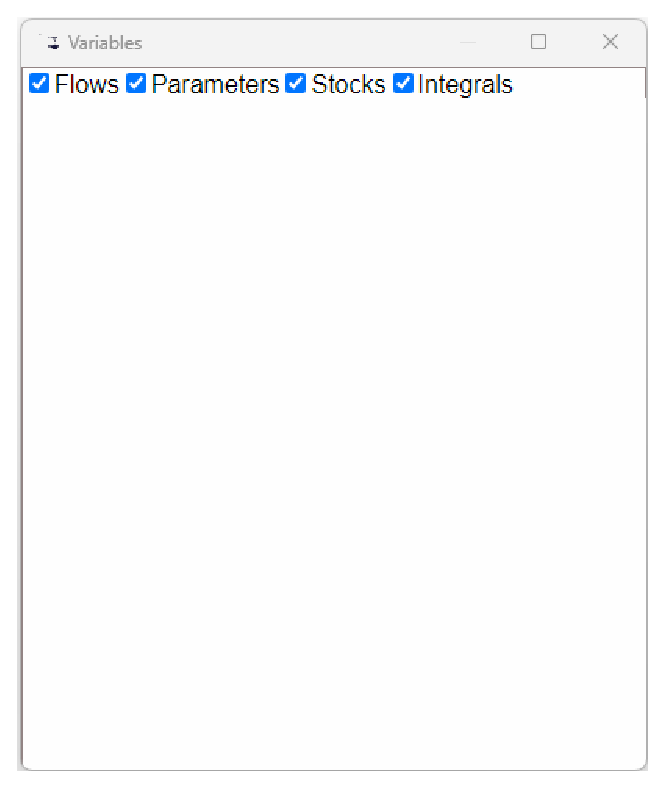
\includegraphics{images/browserWindow}

The browser can be accessed in two ways:
\begin{itemize}
\item From the Insert Menu; or 
\item From the \buttonIcon{var} widget, which brings up a horizontal
menu for defining, constants, parameters and variables. Click on the
final option on this menu, ``Browser'', to bring up the window. 
\end{itemize}
The \emph{variable browser} is a popup window that shows all currently
defined variables in the system. It is an ``always on top'' window,
which will be visible over any other window including those for \emph{Ravel/Minsky}
(and those for other programs which you have open at the time). This
facilitates its use as a means to insert multiple variables into a
model.

This is a convenience toolbar that allows one to select a variable
for insertion into the design canvas, instead of having to type the
new variable's name from scratch.

At the top of the variable browser are some filter checkboxes, that
allow you filter the variables shown by variable type.

\section{Wires}

\label{Wires}

\subsection{Connecting operations with wires}

A wire represents the flow of values from one operation to the next.
To add a wire to the canvas, click on the output port of an operator
or variable (on the right hand side of an icon in its initial unrotated
orientation), and then drag it towards an input port (on the left
hand side of an unrotated icon); an arrow will be drawn out of the
port. The next figure shows an arrow being drawn out of an output
port and dragged towards an input port on a divide block.

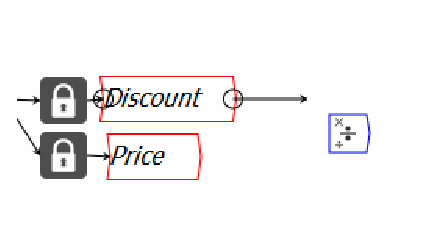
\includegraphics{images/ArrowDrawing01}

When the mouse is released, Ravel searches for a nearby input port
and attaches the wire there.

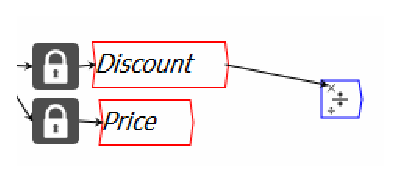
\includegraphics{images/ArrowDrawing02}

When the other variable is wired to the divide operator, the output
can be further processed and allocated to another variable for further
analysis or display.

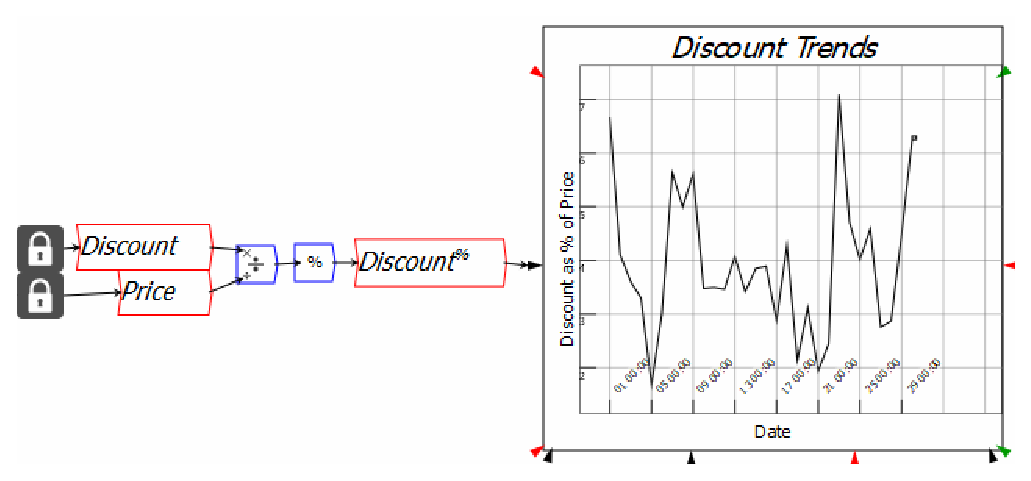
\includegraphics[width=10cm]{images/ArrowDrawing03}

The Equation Tab and LaTeX export shows the equation generated by
this wiring: $\mathrm{Discount}^{\%}=\left(\frac{\mathrm{Discount}}{\mathrm{Price}}\right)$.

You can't connect an operator to itself (that would be a loop, which
is not allowed, unless passing through an integral), nor in general
can an input port have more than one wire attached---the exceptions
are mathematical operators such as $+/-$ and $\times/\div$ (and
similarly max/min), where the multiple wires are summed or multiplied,
respectively.

\subsection{Curving Wires}

A wire can be bent by hovering over it, at which point a blue dots
(``handle'') will appear. Click on the blue dot---or anywhere along
the line---and the line will turn into a curve, with 3 ``bezier''
points showing the degree of curvature.

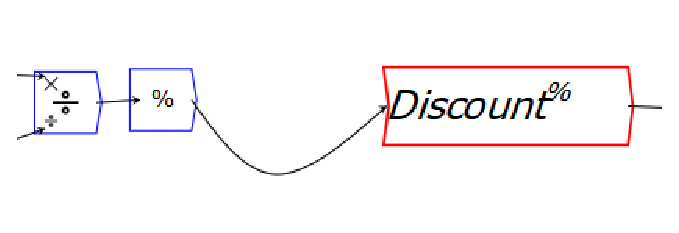
\includegraphics{images/CurvedLine01}

Additional curves can be added to a line, which can allow you to connect
variables without drawing a line across some other entity.

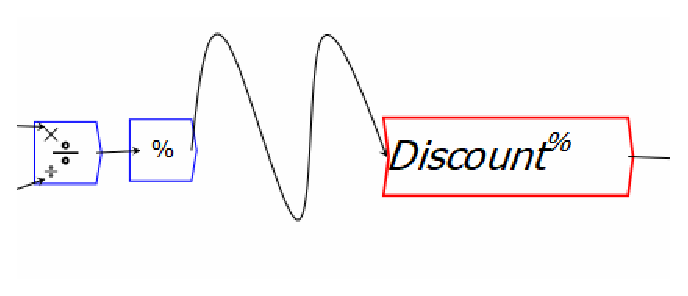
\includegraphics{images/CurvedLine02}

However, it can be preferable to copy a variable and paste into a
document multiple times, rather than having curved wires cluttering
up a diagram. Wires can also become excessively kinked by curving
them, and there is a context-menu command to straighten a curved line.

\section{Groups}

\label{Group}

\operatorKey{group}

Grouping gives the capability to create reusable modules, or subroutines
that can dramatically simplify more complicated systems. Groups may
be created in the following ways: 
\begin{itemize}
\item by lassoing a number of items to select them, then selecting ``group''
from the canvas context menu, or the edit menu. 
\item by pasting the selection. You may ``ungroup'' the group from the
context menu if you don't desire the result of the paste to be a group. 
\item by copying another group 
\item by inserting a Minsky file as a group 
\end{itemize}
Groups are ``transparent'': at a low level of magnification, the
group icon is shown, but as you zoom in on a group, it will become
transparent, which allows you see and edit its contents. 

Groups may be nested heirarchically, which gives an excellent way
of zooming in to see the detail of a model, or zooming out to get
an overview of it. The group context menu item ``Zoom to display''
zooms the canvas in just enough for the group's contents to be visible.

You may also select ``Open in canvas'' from the context menu. This
replaces the current canvas contents with the contents of the group,
allowing you to edit the contents of the group directly without the
distractions of the rest of the model. Select ``Open master group''
to return to the top level group occupying the canvas.

Around the edges of a group are input or output variables, which allow
one to parameterise the group. One can drag a variable and dock it
in the I/O area to create a new input or output for the group.

When creating a group, or dragging a variable or operation into or
out of a group, if a wire ends up crossing the group boundary, a new
temporary variable is added as an I/O variable. You may then edit
the I/O variable name to be something more meaningful to your model.

Variable names within groups can be locally scoped to that group.
That means that a variable of the same name outside the group refers
to a different entity completely. By default, grouped variables refer
to entities outside the group scope, but may be marked local by means
of context menu option. One can also convert all variables in a group
to be local by means of the ``Make subroutine'' context menu entry.

Nonlocal variables refers to a local variable within an outer scope,
going all the way to global scope if no such variable exists. In this
way, two groups can share a variable reference to a variable, and
you can limit the scope of the shared variable by placing a local
variable of the same name in an outer group that both groups are contain
within.

A group can also be exported to a file from the context menu. This
allows you to build up a library of building blocks. There is a github
project ``minsky-models'' allowing people to publish their building
blocks and models for others to use. In the future, we hope to integrate
\emph{Minsky} with this github repository, allowing even more seamless
sharing of models.

\section{Plot widget}

\label{PlotWidget}

\operatorKey{plotWidget}

The plot widget embeds a plot into the canvas.

Around the outside of the plot are a number of input ports that can
be wired:
\begin{itemize}
\item left hand edge Multiple series can be plotted by attaching them as
inputs to the black input triangle on the middle of the Y1 axis.
\item right hand edge Multiple series can be plotted by attaching them
as inputs to the red input triangle on the middle of the Y2 axis.
These are shown on a different scale to the left hand Y1 inputs, which
allows very different magnitudes to be compared on the one plot. 
\item bottom edge The default for the X-axis is either time---for a \emph{Minsky}
simulation model---or the right-pointing axis of a Ravel. XY plots
can be created by attaching an input to the matching input on the
X axis: the input to the black triangle will be plotted against the
variable(s) inputted on the black Y1 input port; and the input to
the red triangle will be plotted against the variable(s) inputted
on the red Y2 input port.
\begin{center}
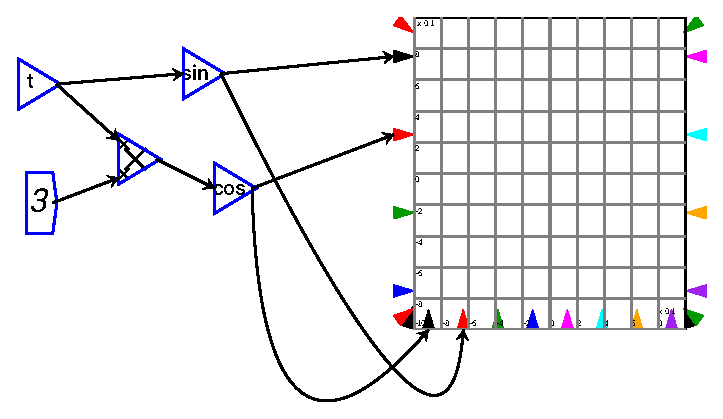
\includegraphics{images/plotLissajous} 
\par\end{center}

If only one bottom port is connected, then that controls all pens
simultaneously, and if no ports are connected, then the simulation
time is used to provide the $x$ coordinates 
\item corners Corner ports control the scale. You can wire up variables
controlling minimum and maximum of the $x$, $y$ and right hand $y$
axes. If left unwired, the scales are determined automatically from
the data---or set by fields in the Options form. Corner ports can
also be used to, for example, implement a sliding window graph---so
that the scale of the graph adapts to the simulation in a \emph{Minsky}
model.
\begin{center}
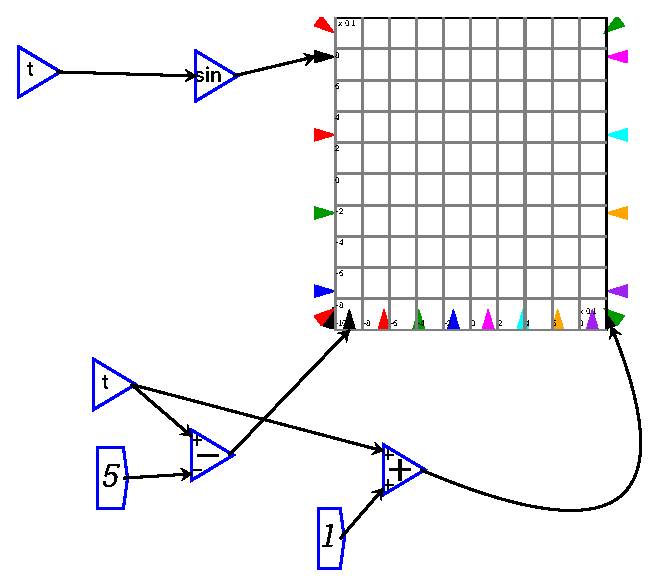
\includegraphics{images/plotSlidingWindow} 
\par\end{center}

\end{itemize}
Plots can be resized using the resize arrows that appear when the
mouse hovers over a plot. Click on one of these arrows and drag the
mouse and the plot will be resized.

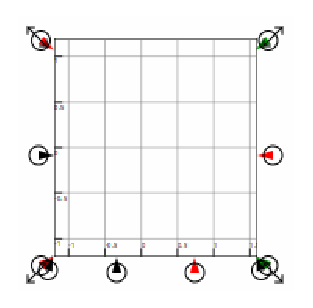
\includegraphics{images/plotResize}

\subsection{Plot context menu}

The plot context menu is:

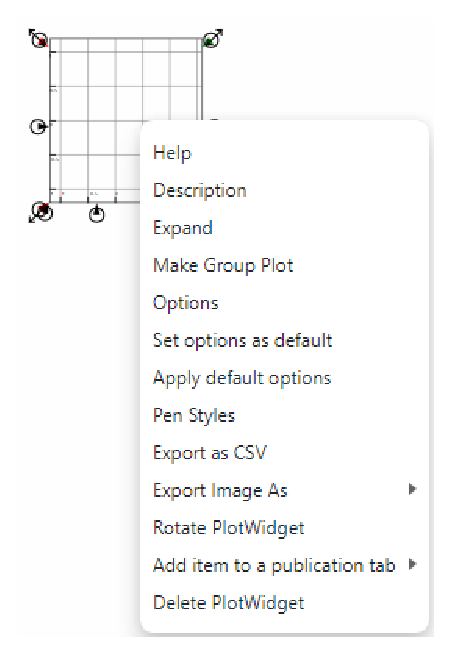
\includegraphics{images/PlotContextMenu}

\subsubsection{Description}

Description bring up a \htmlref{text window}{Notes} into which you can
enter text to describe a plot. The Short Description field becomes
a ``Hint'' that is displayed when the mouse hovers over a plot.
If you check the Bookmark field, the Short Description becomes a bookmark
which can be used to navigate the document.

\subsubsection{Expand}

This generates a large display window for the plot alone, independent
of the \emph{Ravel/Minsky} canvas itself.

\subsubsection{Make Group Plot}

If this option is checked on a plot within a Group, this plot replaces
the default image for a Group. It is a dynamic rendition, so in a
\emph{Minsky} model, this can show the plotted variables changing
over time.

\subsubsection{Options}

The format of a plot is controlled by the Plot Window Options form.
Titles, axis labels, plot type and other features of a plot are controlled
through this form.
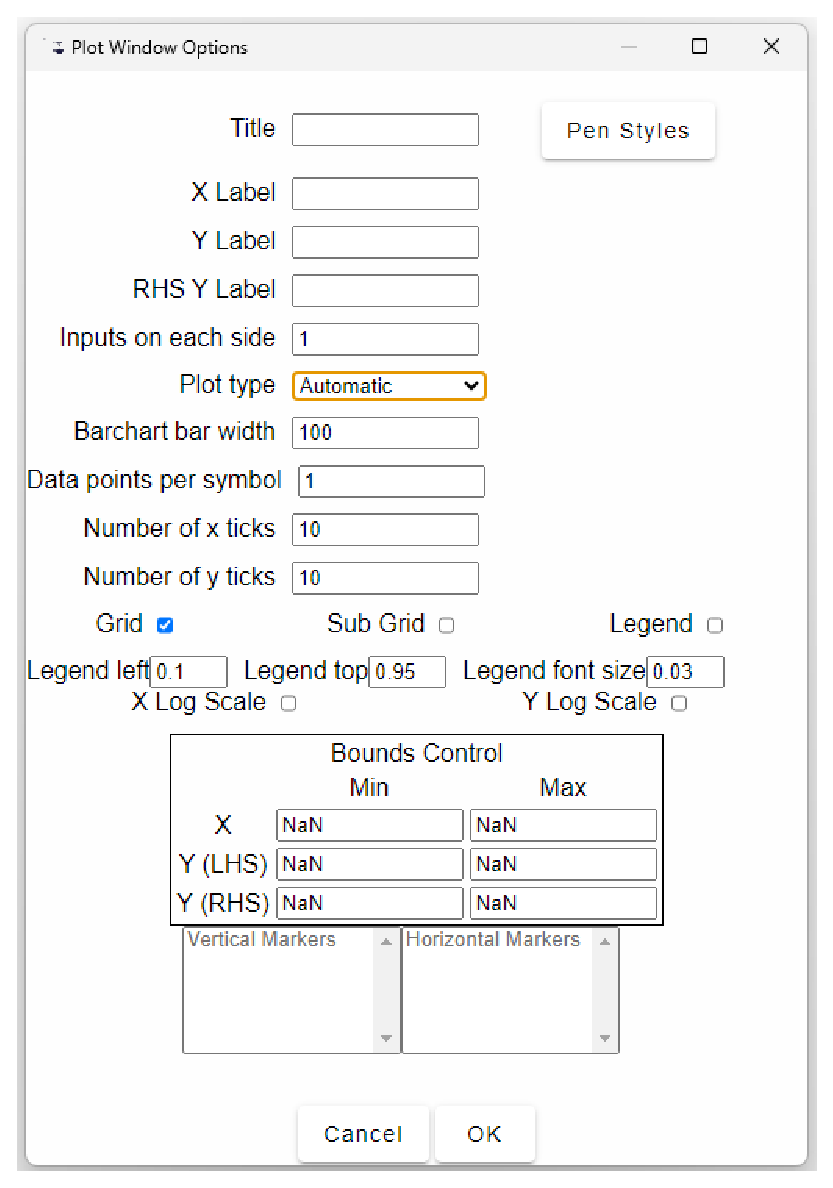
\includegraphics[height=0.9\textheight]{images/plotOptions}

\subsubsection{Set options as default}

This command reproduces the settings of the selected plot in any subsequent
plot. This can expedite plot labelling, as well as setting a default
appearance for the style of graph applied to the data in each plot.

\subsubsection{Apply default options}

This applies the default plot options to any selected plot.

\subsubsection{Pen Styles }

This brings up the pen styles control form. When variables are attached
to the input ports, their names will appear above each formatting
bar. This menu can also be accessed from the Pen Styles button on
the Options form.

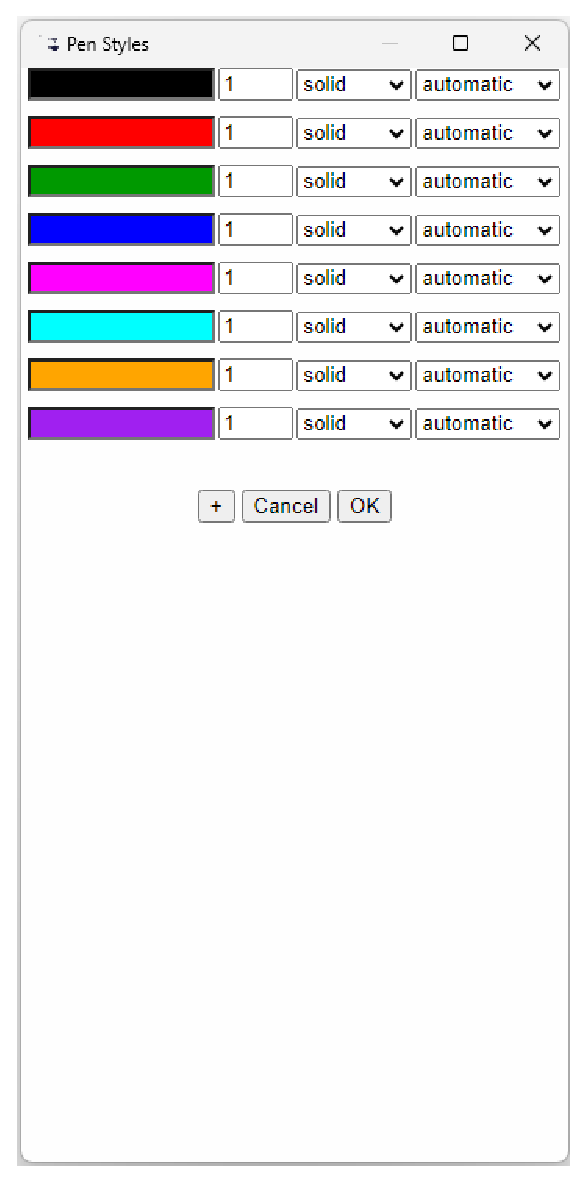
\includegraphics[height=0.65\textheight]{images/PlotPenStyles}

\subsubsection{Export as CSV}

This command exports the data from a Plot as a csv file.

\section{Sheet Widget}

\label{Sheet}

\operatorKey{sheet}

The Sheet widget displays data as in a typical spreadsheet program.

The default sheet is a blank square box, as shown above. Once data
is attached to the sheet, formatted and hierarchical data will fill
the sheet. The example shown below has 4 dimensions---the data is
Price, while the dimensions are Date, Salesperson, Suburb and Source.
Data for the first two dimensions---the downward and right-pointing
Ravel axes---is shown, while the first entry in the third and higher
order dimensions are shown at the head of the sheet. You can alter
the displayed data by manipulating the Ravel attached to the sheet.

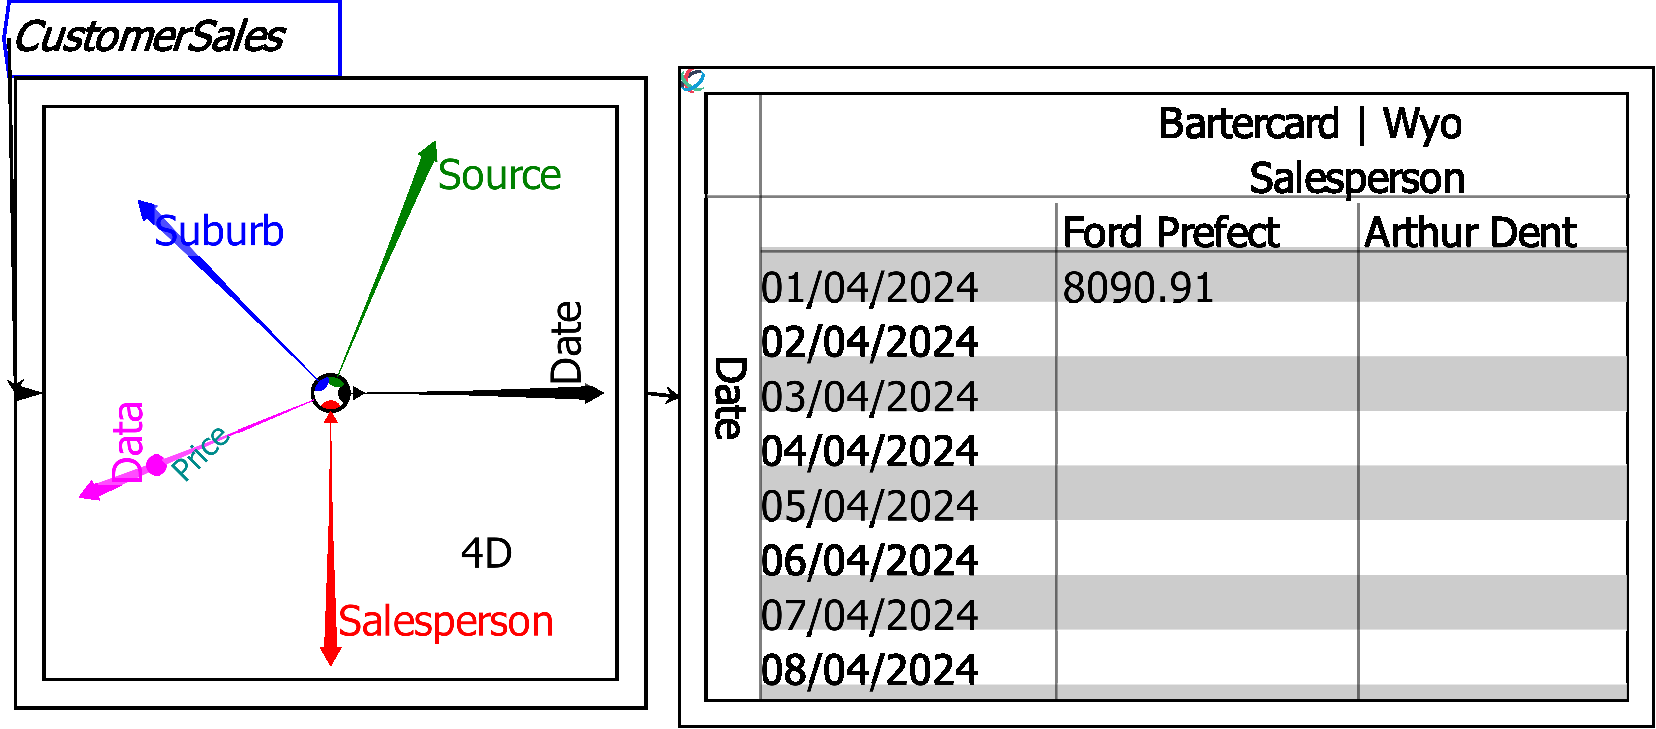
\includegraphics[width=\textwidth]{images/sheetBasics}

To use the Sheet widget, simply attach a variable or Ravel to it via
a wire. The input is on the left-hand side of the sheet widget box.
This sheet displays the input data as a number (in the case of a variable
being simulated in a \emph{Minsky} model) or an array of data (in
the case of a Ravel). Note that only one wire can be connected to
a sheet, as the sheet can only display a single input value--however,
the \emph{Ravel} operators \htmlref{\emph{meld}}{Operation:meld} and
\htmlref{\emph{merge}}{Operation:merge} enable
you to combine data from several Ravels to allow them to be displayed
in a single sheet.

By default, a Sheet outputs the beginning of the data series. The
context menu allows you to specify that the data displayed comes from
the Head of the data (the default), its Tail (the final entries in
the data series), or the Head and Tail. The next figure shows the
Head and Tail displayed for the rows of this sheet.

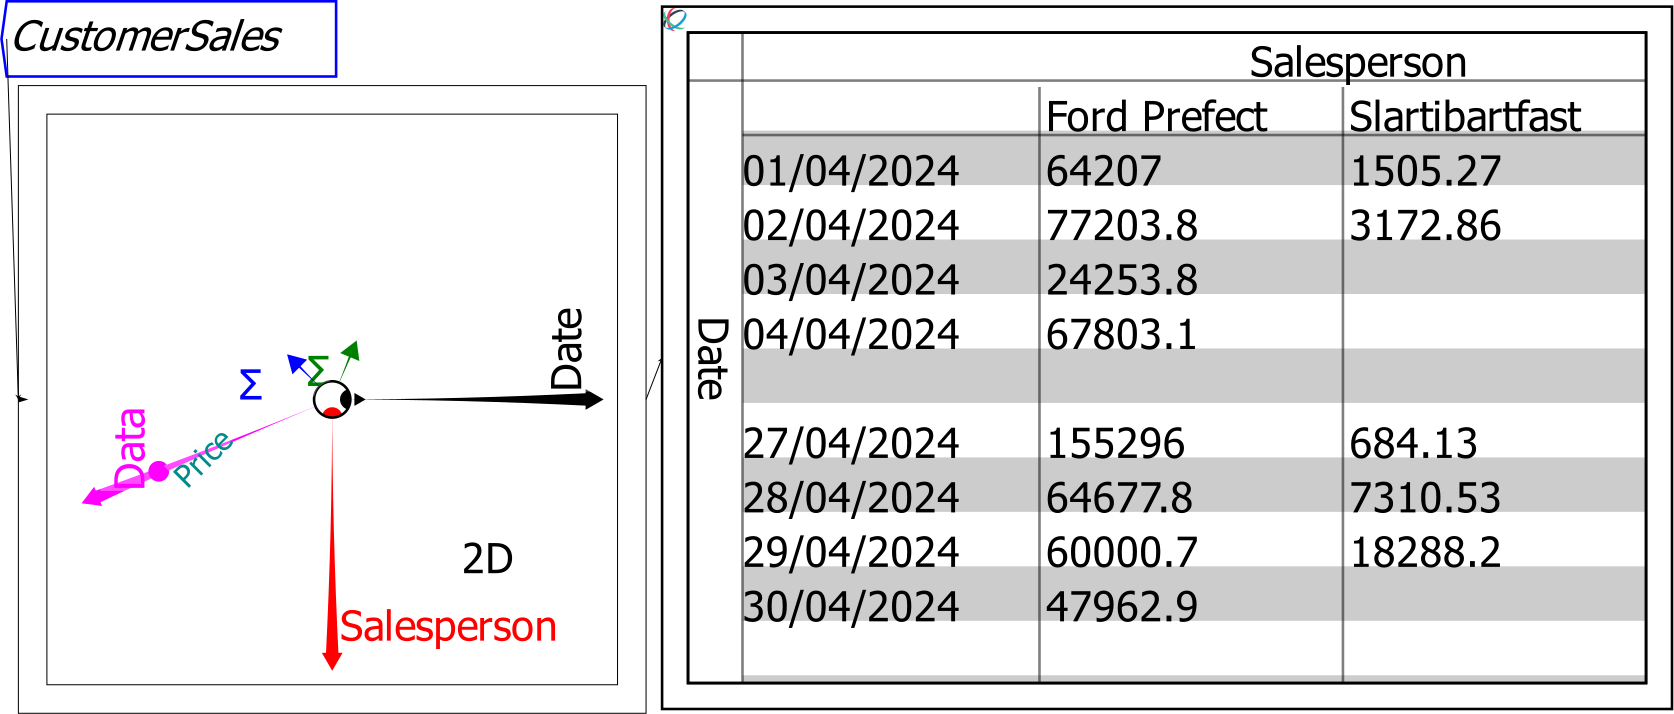
\includegraphics[width=\textwidth]{images/SheetHeadTailSmallBusiness}

\section{Note Widget}

\label{Notes}\label{Item}

\operatorKey{NoteWidget}

The note widget places the text line ``Enter your note here'' on
the canvas.


\includegraphics{images/note}

Double-clicking on the text, or choosing Description from the context
menu, brings up the note form:

\noindent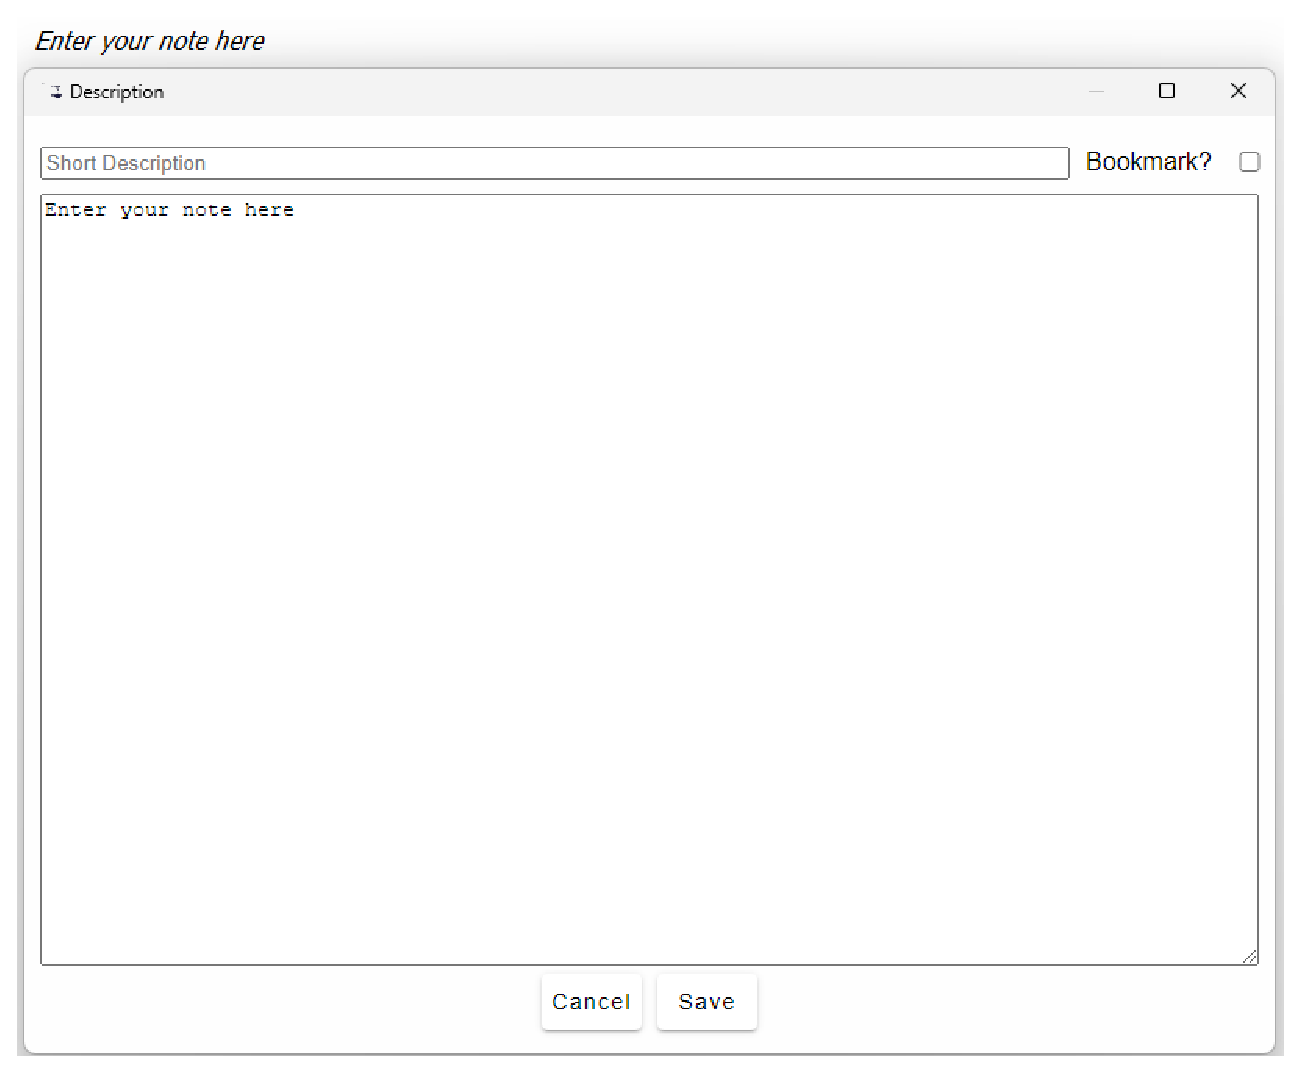
\includegraphics[width=\textwidth]{images/NoteWindow}

The Short Description field becomes a tool-tip for this note, and
also doubles as a \htmlref{Bookmark}{Bookmarks} should you check the
Bookmark? box. 

Notes allow arbitrary text to be placed on the canvas for explanatory
purposes. Anything that can be entered on the keyboard can be placed
here, including unicode characters, and \LaTeX{} formatting is supported. 

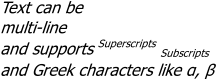
\includegraphics{images/Note+Text}

\section{Context Menu}

All canvas items have a context menu, accessed by clicking the right-mouse
button while hovering over an item, which allow a variety of operations
to be applied to the canvas item. Common context menu items are explained
here: 
\begin{description}
\item [{Help}] bring up context specific help for the item 
\item [{Description}] Attach an annotation to the item. This is only visible
by selecting the description item from the context menu, although
whatever is set as the ``Short Description'' will also appear as
a tooltip whenever the mouse hovers over the item. 
\item [{Port values}] When running a simulation, you can drill down into
the actual values at the input and output ports of the variable or
operation, which is a useful aid for debugging models. 
\item [{Edit}] set or query various attributes of an item. This function
can also be accessed by double clicking on the item. (Plot widgets
behave slightly differently: double-clicking on a plot brings up an
independent window in which the plot is displayed.). 
\item [{Copy}] Creates a copy of an item, retaining the same attributes
of the original. This is very useful for creating copies of the same
variable to reduce the amount of overlapping wiring in a model. This
can substantially improve the readability of a \emph{Ravel/Minsky}
model when compared to standard system-dynamics programs.
\item [{Flip}] actually rotates an object through $180^{\circ}$. You can
specify aribtrary rotations of objects through the edit menu. 
\item [{Delete}] delete the object. 
\end{description}
Item specific context menu items: 
\begin{description}
\item [{variables, parameters and constants}] %
\mbox{%
%
} 
\begin{description}
\item [{Local}] Make the variable's scope local to its \htmlref{group}{Group} 
\item [{Find definition}] Place a red circle on the variable that defines
its value. 
\item [{Select all instances}] Select all instances of this variable 
\item [{Rename all instance}] Do a global search and replace of this variable
name with a new name. 
\item [{Export as CSV}] Export the current variable's value as a CSV file.
\item [{Add integral}] attach an integration operation, and convert the
variable into an integral type.
\end{description}
\item [{integrals}] %
\mbox{%
%
} 
\begin{description}
\item [{Copy Var}] copy just the integrated variable, but not the integration
operation itself.
\item [{Toggle Var Binding}] Normally, integrals are tightly bound to
their variables. By toggling the binding, the integral icon can then
be moved independently of the variable it is bound to. 
\end{description}
\item [{Godley tables}] %
\mbox{%
%
} 
\begin{description}
\item [{Open Godley Table}] opens a spreadsheet-like window to allow financial
flows to be defined in a Godley Table (these can also be defined directly
on the canvas when a Godley Table is displayed in Edit Mode).
\item [{Resize Godley Table}] allows the icon to be resized. 
\item [{Edit/Copy var}] allows individual stock and flow variables to
be copied or edited. 
\item [{Export to file}] export table contents as either CSV data, or
as a \LaTeX{} table, for importing into other software, such as a spreadsheet
or word processor. 
\end{description}
\item [{Groups}] %
\mbox{%
%
} 
\begin{description}
\item [{Zoom to Display}] Zoom the canvas sufficiently to see the contents
of the group. 
\item [{Resize}] Resize the group icon on the canvas. 
\item [{Save group as}] Save the group in it's own Minsky file. 
\item [{Flip contents}] Rotate each item within the group by 180$^{\circ}$ 
\item [{Ungroup}] Ungroup the group, leaving its contents as icons on the
canvas. 
\item [{contentBounds}] Draws a box on the canvas indicating the smallest
bounding box containing the group items. 
\end{description}
\item [{Plot Widgets}] %
\mbox{%
%
} 
\begin{description}
\item [{Expand}] By double-clicking, or selecting ``Expand'' from the
context menu, a popup window is created of the plot, which can be
used examine the plotting in more detail.
\item [{Resize}] Allows you to resize the plot icon on the canvas 
\item [{Options}] Customize the plot by adding a title, axes labels and
control the number of axis ticks and grid lines on the detailed plot.
You can also add a legend, which is populated from the names of variables
attached to the plot. 
\end{description}
\end{description}

\section{Canvas background and keyboard shortcuts}

The canvas is not simply an inert place for the canvas items to exist.
There is also a background context menu, giving access to the edit
menu functionality such as cut/copy/paste, and also keyboard entry.

Special keys: %
\begin{tabular}{rl}
F1  & context sensitive help\tabularnewline
Shift  & enter panning mode\tabularnewline
$\leftarrow,\rightarrow,\uparrow,\downarrow$  & adjust sliders, adjust Ravel slicers\tabularnewline
\end{tabular}

The following keystrokes insert an operation

\begin{tabular}{rl}
  \verb-+- & add\\
  \verb+-+ & subtract \\
  \verb+*+ & multiply\\
  \verb++/ & divide\\
  \verb+^+ & pow\\
  \verb+%+ & percent operator\\
  \verb+&+ & integral\\
  \verb+=+ & Godley table\\
  \verb+@+ & plot\\
  \verb+#+ & start a text comment, finish with return\\
\end{tabular}

Typing any other character, followed by the Return key, will insert
an operation (if the name matches), or otherwise a variable with that
name.

\section{Bookmarks}

Bookmarks are a useful feature for saving the current position and
zoom of the canvas, to be able to come back to that part of the canvas
later. This helps to manage more complicated models. To create a new
bookmark, click on the ``Bookmark'' tab in the top left-hand corner
(in-between ``Edit'' and ``Insert'') and select ``Bookmark this
position''. The program will provide a dialogue box to enter in a
name for the new bookmark. After creating the bookmark, all user-created
bookmarks can be seen in the Bookmarks menu. To delete a bookmark,
simply select ``Delete'' from the Bookmarks menu and select the
desired bookmark. To open an existing bookmark, select one from the
menu.

You may also create a bookmark from any item on the canvas by selecting
the bookmark checkbox in the ``description'' dialog. This is especially
useful with text boxes, since they provide a visual indicator for
what is bookmarked at a given location---Parameter definitions, Plots,
etc.

\section{Dimensional Analysis}

\label{dimensional analysis}

Dimensional analysis is the idea of attaching units of measurement
(eg metre or second) to the quantities being computed. It provides
an additional constraint that the system must satisfy, reducing the
chance of wiring errors. Two different units being added together
will throw up an error --- you cannot add 2 metres to 3 kilograms. But
it should be possible add 2 metres to 3 feet, and get the correct
answer. You may need to explicitly add a multiply operation to convert
from one unit to another, for example, dividing the 3 feet by 3.281
before adding it to the 2 metres, providing a total of 2.914 meters.

\textbf{Using Dimensional Analysis in }\textbf{\emph{Minsky}}

To attach units to quantities in \emph{Minsky}, you use the units
field of the variable/parameters/constants edit dialog box. Each word
typed in this box describes a separate unit. \verb+^+
followed by an integer is used to represent a power. Finally, a single
``/'' indicates that the following units are on the denominator,
dividing the first set of units by the second. So to represent the
unit of acceleration, you can equivalently type all of the following:
\begin{itemize}
\item \verb+m/s^2+ 
\item \verb+m/s s+ 
\item \verb+m/s^-2+ 
\end{itemize}
Or spelling it out in full:
\begin{itemize}
\item \verb+metre/second^2+ 
\item \verb+metre second^-2+ 
\item \verb+metre / second second+ 
\end{itemize}
Note that metre and m are distinctly different units in \emph{Minsky}.

Note -- setting the time dimension is done in the \htmlref{simulation menu}{RungeKutta}.

All function objects require dimensionless inputs. You can use dimensional
analysis to avoid, for example, incorrectly feeding a degree measurement
into a sine function, by requiring them to be multiplied by a radiansPerDegree
parameter.

\section{Tensor values}

\label{tensors}\index{tensors}

Tensors are arrays of data, where the rank of the tensor tells how
many dimensions the data has. A single number (a scalar) has a tensor
of rank 0. A tensor of rank 1 is a column or row of numbers---a vector.
A rank 2 tensor appears is a 2D sequence of numbers (a matrix), for
example:

\[
\left(\begin{array}{ccc}
x & x & x\\
x & x & x\\
x & x & x
\end{array}\right)
\]

A tensor of rank 3 will appear as a three-dimensional cube, rank 4
as a four-dimensional hypercube, and so on. Tensor variables can be
created and used in \emph{Minsky}, but power analysis of multidimensional
data requires the installation of \emph{Ravel}.

\subsection{x-vectors}

When two or more tensors are combined with a binary operation (such as
addition or multiplication), they must have the same rank. For
example, two tensors of rank 2 can be multiplied together, but a
tensor of rank 2 and a tensor of rank 3 cannot. They may have
differing dimensions, which means the values within each tensor may
not necessarily match up 1-to-1 exactly.  To understand what happens
when a given dimension is mismatched requires understanding the
concept of an x-vector\index{x-vector}\label{x-vector}.

When Minsky is given tensor values, it sorts the values within each
tensor by corresponding dimensions. For example, a rank 2 tensor would
have its values sorted into two sets of data. This data can be in the
form of numbers, dates (time values), or strings. Minsky will then
look at cross-sections of the datasets in order to process the values
within. When the dimensions of two tensors match up, for example two
rank 2 tensors, the corresponding cross-sections of both tensors
should also match up. When they don't, a weighted interpolation of the
corresponding values is taken. This involves using an x-vector.

An x-vector is a vector of real values, strings or date/time values.
If no x-vector is explicitly provided, then implicitly it consists of
the the values $(0,\ldots,n_i-1)$, where $n_i$ is the dimension size
of axis $i$ of the tensor.

For example, if the first tensor consists of three elements
$(x_0, x_1, x_2)$ and the second consist of a number of different
elements that roughly correspond to the same three elements, these can
be added together.  The x-vector starts with the first tensor's value
of $(x_0)$ and looks for a matching value in the second tensor. If it
can't find a direct match, it will search for nearby values which
roughly correspond. It can then take those values and interpolate the
corresponding value based on where in the tensor it appears. This is
weighted, so say there are four values nearby, the program will
average those out and find where a value in the middle of those four
values would appear, and what that hypothetical value would be. To
take another example:

Suppose the first tensor was a vector $(x_0,x_1)$ and had an x-vector
(1,3) and the second tensor $(y_0,y_1,y_2)$ had an x-vector (0,2,3),
then the resulting tensor will be $(x_0+0.5(y_0+y_1), x_1+y_2)$. If
the x-vector were date/time data, then the tensor values will be
interpolated according to the actual time values. If the first
tensor's x-vector value lies outside the second tensor's x-vector,
then it doesn't result in a value being included in the output. The
resultant x-vector's range of values is the intersection of input
tensors' x-vector ranges.

If both tensor had string x-vectors, then the resultant tensor will
only have values where both input tensors have the same string value
in their x-vectors. In the above case, where the x-vectors were
('1','3') and ('0','2','3') the resulting tensor will be the scalar
$x_1+y_2$.

It goes without saying that the type of the x-vector for each axis
must also match.



\section{Ravel}

\label{Ravel}\emph{Ravel} the program is a commercial data analysis
extension to the Open Source system dynamics program \emph{Minsky}.
It inherits all of \emph{Minsky}'s features and adds the
Ravel\texttrademark,
% removed \textcircledP as it refers to sound recordings only. Ravel
% is not a sound recording.
%\textcircledP
a graphical object for the manipulation and analysis of multidimensional
data. If you are using \emph{Minsky} and would like to check out \emph{Ravel},
go to \htmladdnormallinkfoot{\emph{Ravel}'s Patreon
  page}{https://www.patreon.com/hpcoder} and
sign up. The monthly fee is US\$7, and there is a
7-day trial period during which you can experiment with using \emph{Ravel}
before the fee is applied.

\subsection{Installing Ravel}

Once you are a member of \emph{Ravel}'s Patreon group, you have access
to the Ravelation Patreon store, and you can download the latest copy
of \emph{Minsky}---either from the store or from attachments to posts
announcing updated versions.

Download and install \emph{Minsky}, which will launch the program
once it is installed. Then choose ``Upgrade'' from the File menu.
The RavelUpgrader form will pop up, asking you for confirmation that
you are willing to let the process check your name and account details
on Patreon.

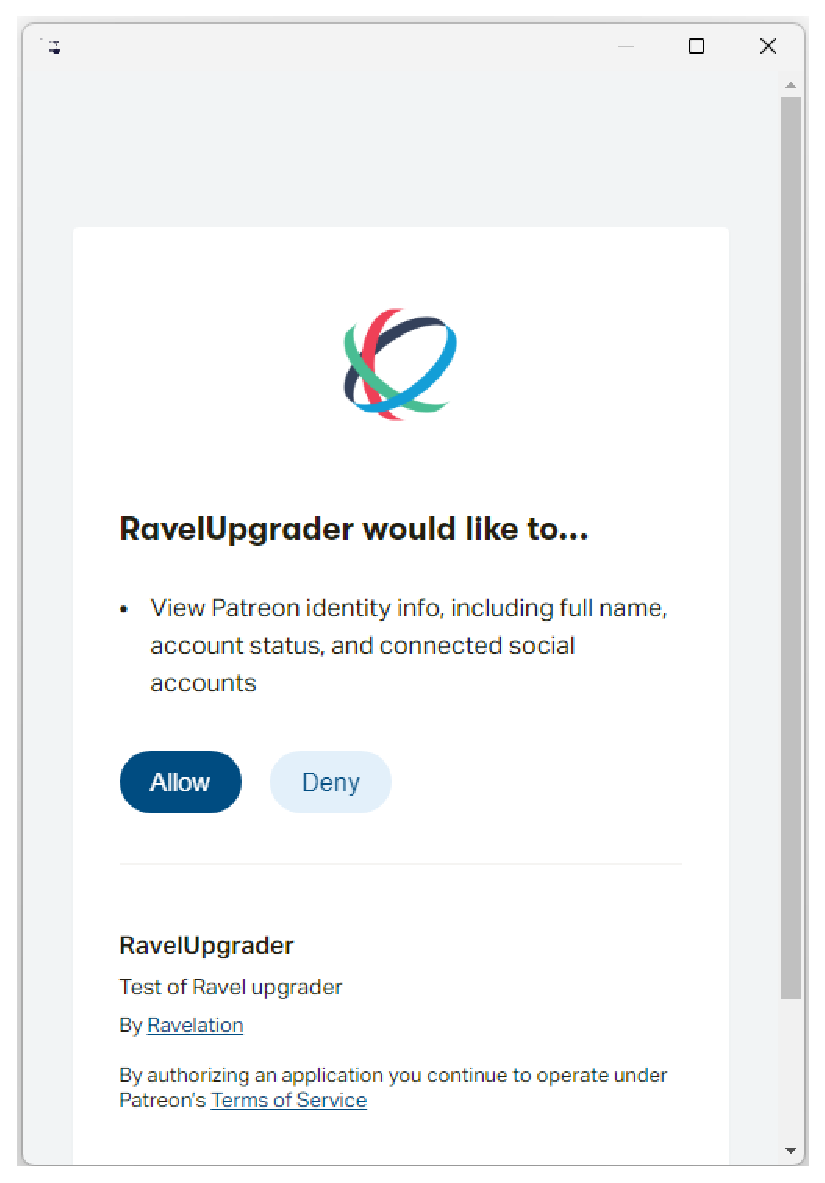
\includegraphics{images/RavelUpgradeForm}

Click on ``Allow'' and \emph{Minsky} will check that you are a member,
and if so then download and install the \emph{Ravel} extension into
\emph{Minsky}. Once this is completed, the latest version of \emph{Ravel
}will be installed in your \emph{Minsky }subdirectory, and you will
have full access to its commands.

\subsection{Introduction to the Ravel GUI Object}

\label{Ravel-GUI Object}

A Ravel is inserted onto the wiring canvas by clicking on the \buttonIcon{RavelIcon}widget
from the toolbar. The first Ravel inserted into a document appears
in Edit mode as shown below, with indicative Axis names:

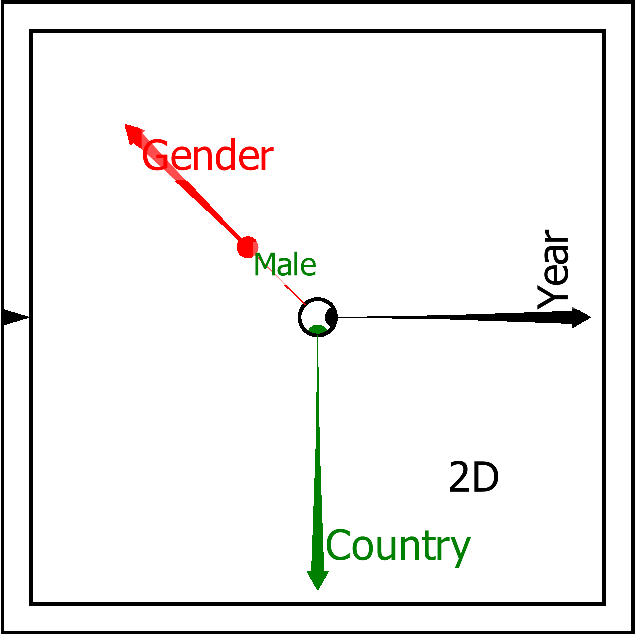
\includegraphics{images/RavelBlank}

The essential step in using a Ravel is to attach data to it via the
triangular input port. See \htmlref{importing CSV files}{CSV import}
for how to import data.  When a data file is attached to the input
port of a Ravel, a multi-arrowed object fills the Ravel rectangle. If
there are seven dimensions or more to the data, it will appear as
shown below, with arrows in a pastel shade and axes labels not shown
unless your mouse is hovering over an axis:

\begin{center}
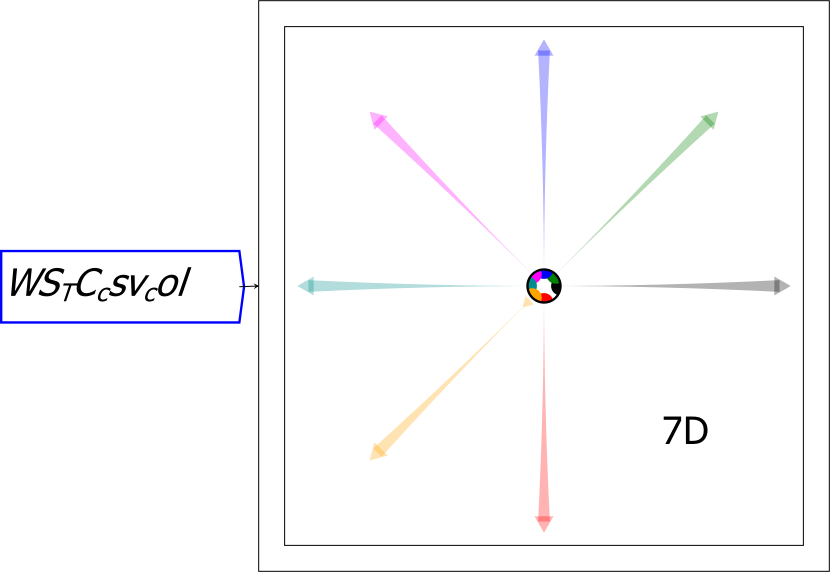
\includegraphics[width=.7\textwidth]{images/RavelDataImporting01}
\end{center}

With six or fewer dimensions it will appear as shown below, with full-colour
axes and axis labels shown:

\begin{center}
  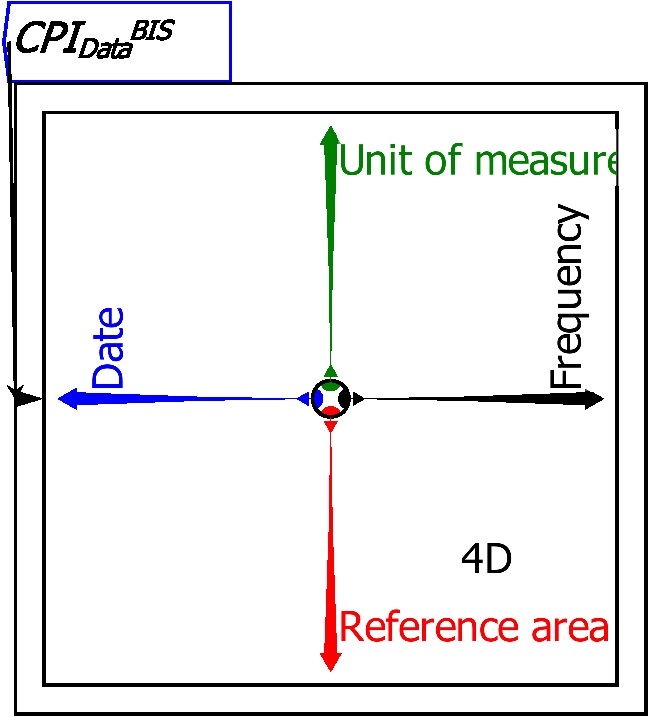
\includegraphics[width=.7\textwidth]{images/RavelDataImporting02}
\end{center}

The arrows are the dimensions of the data; the dots are selectors
for specific values on each dimension. When a \htmlref{CSV import parameter}{CSV import} is first attached to a Ravel, all the selector
dots are in the centre of the Ravel, so that all the data in the Ravel
is output to any Variable, Sheet or Plot attached to it. The next
figure shows all 4 selectors being used so that the Ravel outputs
the annualized rate of inflation for the USA in June 2022.

\noindent\includegraphics[width=\textwidth]{images/RavelSingleDataPointSelected}

If the selector dot remains in the centre for one dimension, then
a column of data for that dimension is output from the Ravel:

\noindent\includegraphics[width=\textwidth]{images/RavelDataSeriesSelected}

With two selector dots remaining in the centre, an array of data is
output. This results in multiple countries' inflation rates being
plotted:

\noindent\includegraphics[width=\textwidth]{images/RavelData2SeriesSelected}

Clearly a number of countries had extreme rates of inflation at various
times between the 1970s and the mid-1990s. There are Ravel functions
which can be used to isolate these countries (see \htmlref{\emph{Operations}}{Operations}),
but it is also easy to identify them visually by moving the selector
dot along the Reference Area axis. You can do this by either:
\begin{itemize}
\item Clicking on the selector dot with the mouse and dragging it along
the axis; or
\item Hovering the mouse over the axis and using the arrow keys. The up-arrow
and right-arrow move you forward along a data axis from the first
entry to the last; the down and left arrow keys move you backward.
\end{itemize}
Eyeballing the data indicates that a 40\% annual inflation rate is
the dividing line between countries which did and did not experience
a hyperinflation in the post-WWII period (defined as from 1955 onwards
to exclude WWII-influenced price disturbances---for instance, those
associated with the Russian occupation of Austria ending in 1955).
That set of countries (Argentina, Brazil, Bulgaria, Chile, Colombia,
Croatia, Czechia, Estonia, Iceland, Indonesia, Israel, Latvia, Lithuania,
Mexico, North Macedonia, Peru, Philippines, Poland, Romania, Serbia,
Slovakia, Slovenia and Turkey) are identified in the next figure as
``HyperInflation'' countries, while the remainder are ``NormalInflation''
countries. Except for Iceland, Israel, the Philippines, and Turkey,
the hyperinflation countries were either South American, or countries
which underwent the transition from socialism to capitalism in the
1990s. This figure also shows the iconized version of a Ravel, which
is generated by toggling ``Editor mode'' on the context menu (also,
by default, the first Ravel inserted into a document is in Editor
mode, and all subsequent Ravels are inserted in iconized mode).

\includegraphics[width=15cm]{images/RavelDataLockedSubsets}

This selection employed one context-menu feature of a Ravel---``Pick
Axis Slices'' was used on the Reference area axis to choose countries
which had annual inflation rate of above 40\% between 1955 and 2024---and
one Ravel-specific widget, the \htmlref{Lock}{Lock}, which creates a
subset of the data which can be allocated to a variable. The selection
on the Ravel can then be changed without altering the subset selected
by the Lock.

Now that the data is sensibly divided, it is feasible to calculate
average inflation rates for normal countries. This is done by choosing
``Av'' on the context menu command ``Set next aggregation'', and
then dragging the Reference Area axis in to the centre of the Ravel.

\includegraphics[width=15cm]{images/CPI_SubsetsAverages}

It is now possible to compare the inflation of individual countries
to the average for all normal inflation countries. In the next figure,
the USA and Japan were selected using Pick axis slices, and their
data is graphed against the average. This shows that Japan's inflation
rate exceeded America's---and the average---until 1975, after which
Japan's inflation rate has been consistently lower than that of the
USA and the average.

\includegraphics[width=15cm]{images/CPI_SubsetsAverageVsSelection}

\subsection{Ravel-specific capabilities}

Ravels have a range of features controlled by the Ravel itself, the
axes of the Ravel, and context menu commands relevant to the Ravel
and its axes.

\subsubsection{Axis rotation}

A Ravel outputs the data in the right-pointing axis as the series
for graphing in a plot, and as the rows of a sheet. In the previous
figures, Date was the right-pointing axis, which generated a set of
time series for plotting (the data shown on the Y1 axis). In the next
figure, Reference Area is rotated into the right-pointing axis position
in the second plot, which means that Date data now generates the x-axis
information. The y-axis information is therefore the rate of inflation
on a specified date. The second plot in the figure below shows the
annual inflation rates for Japan and the USA at the highest point
for the inflation data since WWII. Since this date follows the \htmladdnormallinkfoot{Oil
Embargo}{https://en.wikipedia.org/wiki/1973\_oil\_crisis} imposed
by OPEC members after the \htmladdnormallinkfoot{Yom Kippur War}{https://en.wikipedia.org/wiki/Yom\_Kippur\_War},
this implies that the main cause of the inflationary surge was the
four-fold increase in oil prices (from US\$2.50 a
barrel to \$10) caused by the embargo.

\includegraphics[width=15cm]{images/CPI_SubsetsAxisRotation}

\subsubsection{Axis aggregation}

Axes can be collapsed as well as rotated, in which case the data on
the axis is aggregated according to the choice made on the ``Set
next aggregation'' Ravel context menu. In the next figure, Price
is chosen on the Data axis, and all other axes apart from Date are
aggregated by the Sum function (the default aggregation method). The
Ravel therefore outputs total sales by date.

\noindent\includegraphics[width=\textwidth]{images/SmallBusinessAggregation}

The available aggregations are: Sum, Product, Average, Minimum, Maximum,
and Standard Deviation. The default setting is Sum. The other options
can be set via the Context (right-mouse click) menu for Ravels.

\subsection{Context menu for Ravels}

\begin{tabular}{|c|p{.7\textwidth}|}
\hline 
Command & Effect\tabularnewline
\hline 
\hline 
Help & Bring up context help on Ravels\tabularnewline
\hline 
Description & Open a text form for documenting the Ravel\tabularnewline
\hline 
Editor Mode & Toggle between seeing the Ravel in Edit or Icon mode\tabularnewline
\hline 
Export as CSV & Export the data in the Ravel as a CSV file\tabularnewline
\hline 
Set next aggregation & Determine the mathematical operation applied when the next axis is
collapsed\tabularnewline
\hline 
Collapse all handles & Aggregate all axes. Ravel will return a single number\tabularnewline
\hline 
Expand all handles & Disaggregate all axes. \tabularnewline
\hline 
Flip & Turn the Ravel around so that the input is on the right and output
on the left\tabularnewline
\hline 
Link specific handles & Control over linked Ravels to link only some aspects--orientation,
caliper, etc.\tabularnewline
\hline 
Join Link Group & Add this Ravel to an existing set of linked Ravels\tabularnewline
\hline 
Unlink & Remove this Ravel from an existing set of linked Ravels\tabularnewline
\hline 
Toggle Axis Calipers & Turn the caliper on a selected axis on or off\tabularnewline
\hline 
Sort Axis & Sort axis by the value of axis labels.\tabularnewline
\hline 
Sort by value & Sort axis by the value of the data on an axis.\tabularnewline
\hline 
Pick axis slices & Manually choose which axis values are output by the Ravel\tabularnewline
\hline 
Axis properties & Description and Dimension show the dimension name; Set next aggregation\tabularnewline
\hline 
Rotate Ravel & Rotate the Ravel through an arbitrary angle\tabularnewline
\hline 
Add to Publication Tab & Place the Ravel on a specified Publication Tab\tabularnewline
\hline 
Delete Ravel & \tabularnewline
\hline 
\end{tabular}

\subsubsection{Calipers}

\label{Calipers}A caliper is a range selector for an axis. Its customary
use will be to select a range of dates, but a caliper can be applied
to any axis to select a subset of data which is contiguous. In the
next figure, calipers have been applied to extract the last 15 days'
of data from this Ravel.

\noindent\includegraphics[width=\textwidth]{images/SmallBusinessCalipers}

When a caliper is initially created, it spans the entire range of
a given dimension. It is applied to sections of that data by moving
the vertical left or right side of the parenthesis; the entire parenthesis
is moved by clicking and dragging on the peak of the parenthesis---the
length of the selection is thus maintained while the segment selected
is altered.

Ravel currently allows one caliper per axis. Future releases will
enable multiple calipers, which will allow non-contiguous segments
of data to be displayed on the one plot or sheet.

\subsubsection{Sort axis}

The default order of an axis is the same as the data input into it.
Once loaded into a Ravel, the data can be sorted by the names of axis
entries---for example, countries can be sorted alphabetically. This
can be sorted forward (from A to Z) or in reverse.

\subsubsection{Sort by value}

The order of an axis can also be determined by the data values for
specific axis selections. The command is only available if the axis
selections return a single column of data for ranking---for example,
in the inflation data, a single date is chosen so that the value of
the inflation for all Reference Areas (countries) can be compared.
There are four options generated by the combination of dynamic or
static sorting, and forward or backward direction. Static sorting
sorts the single axis by the value of the data, and does not alter
that data as (for example) different dates are chosen using the selector
dot. Dynamic sorting alters the order so that the axis is resorted
when (for example) a different date is selected. In the next figure,
dynamic sorting is applied to the Reference Area axis for the rate
of inflation. The output is also put through a \htmlref{Slice}{Operation:slice}
operator, so that only the top 5 countries are output.

\noindent\includegraphics[width=\textwidth]{images/CPI_SubsetsDynamicSorting}

\subsubsection{Pick axis slices}

Pick axis slices lets you select an arbitrary number of slices---as
was done above to choose just the USA and Japan to compare their rates
of inflation. Individual slices can be chosen by left-clicking on
the slice; to select more than one slice, hold down the control key
as you click.

\includegraphics{images/PickSlices}

\subsubsection{Flip Ravel}

This is a convenience command, which is convenient when it would be
preferable to have the output from a Ravel be on its left side rather
than its right--for example, when the Ravel is linked to the Y2 axis
of a plot.

\subsection{Lock}

\label{Lock}

\operatorKey{Lock}

Locks can only be attached to the output of Ravels. The Lock widget
is used to fix the output of a Ravel to a particular configuration
of data. After the Lock is closed (either by double-clicking on the
Lock, or choosing Lock from the context menu), alterations can be
made to the source Ravel without altering the output of the Lock.
This makes it possible to take multiple slices of the data from one
Ravel, and to work with them by assigning those slices to variables,
manipulating the subset of data via additional Ravels, etc. It has
a number of useful context menu commands.

\subsubsection{Apply Lock state to Ravel}

This menu item imposes the lock's state on the source Ravel. Since
many locks can be applied to one Ravel, this makes it easy to edit
the data as required to fine-tune individual locks. For example, the
data for \emph{Inflation}\textsubscript{\emph{Average}}\emph{}\textsuperscript{\emph{Normal}}
initially began in 1950. Since this included a very brief period of
hyperinflation for Austria associated with Russia ceasing its posr-WWII
occupation, it was advisable to alter the selection to start the caliper
in 1955. This was easily done by applying the state of the lock to
the Ravel, then editing the caliper, and opening and re-closing the
lock.

\subsection{Linking Ravels \label{Linking-Ravels}}

When Ravels share dimensions, it is possible to link them together
so that what is done to one Ravel---plotting, selecting data, rotating
axes, etc.---is done to the other Ravel. This is very useful when
you wish to examine relations between different sets of data.

Ravels are linked by dragging the mouse to select the desired Ravels,
then choosing ``Link selected Ravels'' from the context menu when
the mouse is hovering over the canvas.

In the next figure, the two Ravels whose borders are highlighted in
brown have been linked. When the country ``United States'' is chosen
for the Ravel containing house price data, the same selection is made
for the Ravel containing household debt data. The plot and the regression
analysis therefore compare United States house price changes to the
change in the change in household debt.

\noindent\includegraphics[width=\textwidth]{images/RavelLinking}

When the selector dot for Country is moved to another country, the
graph and the correlation result for household debt and house prices
for that country replaces the information shown for the USA.

\noindent\includegraphics[width=\textwidth]{images/RavelLinking2ndCountry}

Linking can be refined using the context menu for Ravels---rather
than for the canvas. If your mouse is over one of the selected Ravels
rather than the canvas, the context menu option is ``Lock specific
handles''. That brings up the detailed lock menu:

\noindent\includegraphics[width=\textwidth]{images/RavelLockSpecificHandles}

It is thus possible to turn on or off selecting of the same slices,
arrow orientation, calipers and sort order if desired, while still
linking the Ravels on other characteristics.

\section{Importing data into a parameter from a CSV file}

\label{CSV import} \index{CSV|import}\label{Operation:csvImport}

After creating a parameter from the ``Variable'' drop-down in the
``Insert'' menu, right-clicking the parameter and selecting the
option to ``Import CSV'', will open a dialogue box that allows you
to select a CSV file. Upon selecting the file, a dialog is opened,
allowing you to specify assorted encoding parameters.

An alternative is to click on the ImportData icon \buttonIcon{importData.eps},
which will create a new parameter for you to import the data into.

The dialog looks somewhat like this (developments in the import routine
may change some layout details):
\begin{center}
\resizebox{\textwidth}{!}{\includegraphics{images/CSVimportDialog}} 
\par\end{center}

\subsection{Quick instructions}

\begin{itemize}
\item Data is typically (but not always) stored in the rightmost columns
of a CSV file. Shift click to set the top left cell of the data. Columns
to the left will be marked as axes. 
\item Select ``axis'' in the Dimension dropdown to include a column as
an axis. Column data turns blue. 
\item Select ``ignore'' in the Dimension dropdown to exclude a column.
Column data turns red. 
\item Select ``data'' in the Dimension dropdown to treat a column as a
data column. Column data turns black. 
\item Select Type for included axis columns. Select one of three types: 
\begin{description}
\item [{string}] most general type, data treated as is. 
\item [{value}] value data must be numerical, e.g. 1, 2, and not quoted
(as in ``1'', ``2'', etc.)
\item [{time}] data must refer to date-time data. The format field may
be used to control interpretation of this data, though if this field
is left blank, Ravel will interpret the data format itself. Blank
format assumes data contains year/month/day/hour/minute/second separated
by some non-numerical character. If fewer than 6 numerical fields
present (from year to second), smallest units are set to minimum value
(0 or 1 respectively). 
\end{description}
\item Click the OK button. 
\item Data is imported into the parameter. 
\item You may need to set units for the imported data field, which can be
done via the Edit $\rightarrow$ Dimensions menu item.
\end{itemize}
In the case shown above, the system has automatically guessed that
the data is 3 dimensional, and that the first 3 columns give the axis
labels for each dimension (shown in blue), and the 4th column contains
the data. The first row has been automatically determined to be the
first row of the file --- with the dimension names are shown in green.

In this case, the automatic parsing system has worked things out correctly,
but often times it needs help from the computer user. An example is
as follows:
\begin{center}
\resizebox{\textwidth}{!}{\includegraphics{images/CSVimportDialogFail}} 
\par\end{center}

In this example, \emph{Ravel} has failed to determine where the data
starts, probably because of the columns to the right of the ``Price''
columns. So the first thing to do is tell it where the data is located.
This is one function of the context menu for data importing. The options
are:

\noindent\begin{tabular}{|c|p{0.5\textwidth}|}
\hline 
Command & Effect\tabularnewline
\hline 
\hline 
Set as header row & Tell Ravel that the selected row contains the header information for
the import\tabularnewline
\hline 
Auto-classify columns as axis/data & Invoke \emph{Ravel}'s automated column classification routine\tabularnewline
\hline 
Populate column labels & Transfer the information from the header row to the Name row\tabularnewline
\hline 
Populate current column label & Transfer the information from the header to the Name for one column
only\tabularnewline
\hline 
Set start of data row, and column & Tell \emph{Ravel }where data begins in the file\tabularnewline
\hline 
Set start of data row & Tell \emph{Ravel} where data begins in the file\tabularnewline
\hline 
Set start of data column & Tell \emph{Ravel} where data begins in the file\tabularnewline
\hline 
\end{tabular}
\begin{center}
\resizebox{\textwidth}{!}{\includegraphics{images/CSVimportDialogSelectData}} 
\par\end{center}

Note that this causes all columns to the right of ``Price paid''
to be treated as data, which is not right, since the columns to the
right of ``Price (text infill)'' are text based columns, not data.
So we need to mark those columns as either ``axis'' or ``ignore''.
To do that, click and drag your mouse on the header field, which will
cause those columns to be selected, like so:
\begin{center}
\resizebox{\textwidth}{!}{\includegraphics{images/CSVimportDialogSelectedColumns}} 
\par\end{center}

Then in the dimensions row, select ``axis'', which flips the selected
columns:
\begin{center}
\resizebox{\textwidth}{!}{\includegraphics{images/CSVimportDialogSelectedAxes}} 
\par\end{center}

Now the axes index labels are rendered in blue, the axes names in
green and the data is in black. In this example, some axes have unique
values, which are not particularly useful to scan over. Other examples
might have columns that duplicate others, for example when the data
has been entered via a database program that allows the user to type
country codes (e.g., LX) rather than the full country name (Luxembourg).
Only one of these axes is needed to uniquely specify the country,
so you can exclude the unwanted dimension by choosing ``ignore''
in the ``Dimension'' row. The deselected columns are rendered in
red, indicating that its data will not be imported into \emph{Ravel}:
\begin{center}
\resizebox{\textwidth}{!}{\includegraphics{images/CSVimportDialogAxesDeselected}} 
\par\end{center}

In this example, the axis names has not been correctly inferred. Whilst,
one can manually edit the axis names in the ``Name'' line, a quick
shortcut is to select ``Populate column labels'' from the context menu. 
\begin{center}
\resizebox{\textwidth}{!}{\includegraphics{images/CSVimportDialogAxesNamed}} 
\par\end{center}

\subsection{Temporal data}

The Date column is current parsed as strings, which not only will
be sorted incorrectly, but even if the data were in a YYYYMMDD format
which is sorted correctly, will not have a uniform temporal spacing.
It is therefore important to parse the Date column as temporal data,
which is achieved by changing the column type to ``time'', and specifying
a format string, which follows strftime conventions with the addition
of a quarter specifier (\verb+%Q+). \index{strftime format specifier}\label{strftime format specifier}

If your temporal data is in the form Y{*}M{*}D{*}H{*}M{*}S, where
{*} signifies any sequence of non-digit characters, and the year,
month, day, hour minutes, second fields are regular integers in that
order, then you can leave the format string blank \index{blank strftime format}.
If some of the fields are missing, eg minutes and seconds, then they
will be filled in with sensible defaults.
\begin{center}
\resizebox{\textwidth}{!}{\includegraphics{images/CSVimportDialogTimeFormat}} 
\par\end{center}

\begin{table}
\begin{tabular}{|c|p{.8\textwidth}|}
\hline 
Code  & Description \tabularnewline
\hline 
\%a or \%A  & The name of the day of the week according to the current locale, in
abbreviated form or the full name.\tabularnewline
\%b or \%B  & The month name according to the current locale, in abbreviated form
or the full name.\tabularnewline
\%d  & Day of month in range 01 to 31\tabularnewline
\%e  & Day of month in range 1 to 31\tabularnewline
\%H  & Hour in range 0 to 23\tabularnewline
\%I  & Hour in range 1 to 12\tabularnewline
\%m  & Month as a decimal number (01 to 12)\tabularnewline
\%M  & Minute in range 00 to 59\tabularnewline
\%Q  & Quarter (0=1st January, 1=1st March etc)\tabularnewline
\%p  & AM or PM\tabularnewline
\%s  & Number of seconds since epoch (1st January 1970)\tabularnewline
\%S  & Seconds in range 00 to 59 \tabularnewline
\%y  & Two digit year YY\tabularnewline
\%Y  & Four digit year YYYY\tabularnewline
\%z  & numerical timezone offset\tabularnewline
\%Z  & Timezone name\tabularnewline
\%\%  & Literal \% character\tabularnewline
\hline 
\end{tabular}\caption{Table of strftime codes}
\label{Strftime code} 
\end{table}

A \emph{Strftime }formatted string consists of escape codes (with
leading \% characters). All other characters are treated as matching
literally the characters of the input. So to match a date string of
the format YYYY-MM-DD HH:MM:SS+ZZ (ISO format), use a format string
``\verb|%Y-%m-%d %H:%M:%S+%Z|''. Similarly, for quarterly data
expressed like 1972-Q1, use ``\verb+%Y-Q%Q+''. Note that only \%Y
and \%y can be mixed with \%Q (nothing else makes sense anyway).

Note that if your month data uses month names instead of numerical
month representation, the it is important you select \%d or \%e
depending on whether your day data has leading zeros or not.  This is
unfortunately a restriction of the underlying date import routine,
which may change in the future.

Even in the current settings, you may still get a message ``exhausted
memory --- try reducing the rank'', or a similar message about hitting
a 20\% of physical memory threshold. In some cases, ``titles'' and
``addresses'' might be pretty much unique for each record, leading
to a large, but very sparse hypercube. If you remove those columns,
then you may encounter the ``Duplicate key'' message. In this case,
you can aggregate over these records---which is desirable anyway
to analyse trends in aggregate data. You do this by setting ``Duplicate
Key Action'' to sum (or perhaps average for this example). After
some additional playing around with dimensions to aggregate over,
we can get the data imported.
\begin{center}
\resizebox{\textwidth}{!}{\includegraphics{images/CSVimportDialogFinal}} 
\par\end{center}

\subsection{Duplicate keys}

In a hypercube, data is indexed by a list of indices, collectively
known as a key. The indices may be strings, integers or date/time
values. If more than one value exists in the CSV file for a given
key, Minsky throws a ``Duplicate key'' exception. This exception
gives you the option of writing a report, which is basically a sorted
version of the original CSV file, with the errors listed at the beginning.
You can open this report in a spreadsheet to see if data needs to
be corrected or removed.

Duplicates will arise if you load data from a transactional database
which stores the exact time of every transaction. Here the correct
choice on ``Duplicate Key Action'' is to sum the entries so that
all sales for a particular day (or month, quarter, or year) are aggregated
for analysis of trends in the data.

\subsection{Counter mode}
\label{counter}

As mentioned previously, Ravel is designed to work with numerical
data. However, it is possible to work with purely symbolic data by
using {\em counter mode}\index{counter mode}. This mode counts the
number of times a key is present in the data file --- either zero or
one, or in the case of duplicate keys, a value greater than one. You
can feed this into a Ravel and perform rollups to analyse the symbols
statistically, for example as histograms.

To select counter mode, select the ``counter'' check box in the input
dialog form. If no data columns are present at all, Ravel
automatically selected counter mode.

\section{Minsky-specific commands}

\subsection{File Menu Minsky commands}
\begin{description}
\item [{Library}] Opens a repository of models for the Minsky simulation
system.
\item [{Recording}] Record the states of a model as it is being built for
later replay. This is useful for demonstrating how to build a model,
but bear in mind that recorded logs are not, in general, portable
between versions of Minsky.
\item [{Replay recording}] Replay a recording of model states.
\end{description}

\subsection{Options Menu Commands}

The options menu allows you to customise aspects of Minsky.
\begin{description}
\item [{Preferences}]~
\begin{itemize}
\item Godley table show values. When ticked, the values of flow variables
are displayed in the Godley table whilst a simulation is running.
This will tend to slow down the simulation somewhat. 
\item Godley table output style --- whether $+/-$ or DR/CR (debit/credit)
indicators are used. 
\item Enable multiple equity columns - whether Godley table have more than
one equity columns. 
\item Number of recent files to display --- affects the \htmlref{recent
files}{recentfiles} menu. 
\item \label{wrap-equations-1} Wrap long equations in LaTeX export. If
ticked, use the breqn package to produce nicer looking automatically
line-wrapped formulae. Because not all LaTeX implementations are guaranteed
to support breqn, untick this option if you find difficulty. 
\item \label{font-1} select a font for variable names etc. 
\end{itemize}
\item [{Background colour}] --- select a colour from which a colour scheme
is computed.
\end{description}

\subsection{Simulation Menu Commands}

\label{RungeKutta}

The Simulation Menu invokes the Simulation Parameters form.

\noindent\includegraphics[width=\textwidth]{images/SimulationParameters}

\begin{itemize}
\item Time unit allows one to specify units for the time dimension for dimensional
analysis. eg ``year'', ``s'' etc. 
\item Min and Max step size control aspect of the adaptive Runge-Kutta equation
solver, which trade off performance and accuracy of the model. The
algorithm is adaptive, so the step size will vary according to how
stiff the system of equations is. 
\begin{itemize}
\item Specifying a minimum step size prevents the system from stalling,
at the expense of accuracy when the step size reaches that minimum. 
\item Specifying a maximum step size is useful to ensure one has sufficient
data points for smooth plots. 
\end{itemize}
\item An iteration is the time between updates to plots. Increasing the
number of solver steps per iteration decreases the overhead involved
in updating the display, at the expense of smoothness of the plots.
\item Start time is the value of the system $t$ variable when the system
is reset. 
\item Run until time can be used to pause the simulation once $t$ reaches
a certain value. Setting this to ``Infinity'' causes the simulation
to run indefinitely, or until some arithmetic error occurs. 
\item The algorithm is adaptive, so the step size will vary according to
how stiff the system of equations is. 
\item Solver order determines how high order a polynomial is used for approximating
the actual system. A first order explicit solver is the classic Jacobi
method, which is the fastest, but least accurate solver. 4th order
is the adaptive Runge-Kutta equation solver.
\end{itemize}

\subsection{Record/Replay Buttons}

\label{RecReplayButtons}

\htmladdimg{recReplayButtons.png}

These buttons control the recording / replay mode of \emph{Minsky}.
You can record your interactions with \emph{Minsky}, and replay those
interactions for demonstration/presentation purposes.
\begin{enumerate}
\item Record a session of building/modifying a model. Note that replaying
a recorded session always starts from a blank canvas, so if you're
recording the modification of a model, ensure that the first thing
recorded is to load the model being modified. This button is a toggle
button, so clicking it again finishes the session, and closes the
file. 
\item Simulate/Replay button. Pressing this button puts \emph{Minsky} into
replay mode, and asks for a recording file. You may use the run buttons
(run/pause,stop and step), as well as the speed slider, to control
the replay. This button is a toggle button, so clicking it again returns
\emph{Minsky} back to the default simulation mode. 
\end{enumerate}

\subsection{Run Buttons}

\label{RunButtons}

\htmladdimg{NewItem15.png}

The Run buttons respectively: 
\begin{enumerate}
\item Start a simulation--when started the button changes to a pause icon,
allowing you to pause the simulation \buttonIcon{NewItem23.png}. 
\item Stop a simulation and reset the simulation time to zero 
\item Step through the simulation one iteration at a time. 
\item Reverse checkbox changes the simulation time direction. Bear in mind
that a simulation will eventually diverge from its original trajectory
due to chaotic effects. 
\end{enumerate}

\subsection{Speed slider}

\label{Speedslider}
\begin{center}
\htmladdimg{NewItem16.png} 
\par\end{center}

The speed slider controls the rate at which a model is simulated.
The default speed is the maximum speed your system can support, but
you can slow this down to more closely observe dynamics at crucial
points in a simulation.

\subsection{Simulation time}

\label{SimTime}

In the right hand top corner is a textual display of the current simulation
time $t$, and the current (adaptive) difference between iterations
$\Delta t$.
\begin{description}
\item [{Time}] \buttonIcon{time.eps} embeds a reference to the simulation
time on the Canvas. This is not necessary in most simulations, but
can be useful if you want to make a time-dependent process explicit,
or control the appearance of a graph.

For example, by default a graph displays the simulation time on the
horizontal axis, so that cycles get compressed as a simulation runs
for a substantial period:
\begin{center}
\resizebox{\textwidth}{!}{\includegraphics{images/NewItem36}} 
\par\end{center}

If a Time block is added to the marker for the x-axis range, you can
control the number of years that are displayed. This graph is set
up to show a ten year range of the model only:
\begin{center}
\resizebox{\textwidth}{!}{\includegraphics{images/NewItem37}} 
\par\end{center}
\item [{Godley Table}] \buttonIcon{NewItem29.eps}. This is the fundamental
element of \emph{Minsky} that is not found (yet) in any other system
dynamics program.

Clicking on it and placing the resulting Bank Icon on the Canvas enters
a Godley table into your model:
\begin{center}
\includegraphics{images/NewItem29} 
\par\end{center}

Double-click on the Bank Icon (or right-click and choose ``Open Godley
Table'' from the context menu) and you get a double-entry bookkeeping
table we call a Godley Table, which looks like the following onscreen:

%\fwhtmladdimg{NewItem30.png}

\begin{center}
\scalebox{0.5}{\includegraphics{images/emptyGodley}} 
\par\end{center}

Use this table to enter the bank accounts and financial flows in your
model. We discuss this \htmlref{later}{Godley-Tables}.
\item [{Integration}] \buttonIcon{int.eps}.\label{Integrate} This inserts
a variable whose value depends on the integral of other variables
in the system. This is the essential element for defining a dynamic
model. Click on it and the following entity will appear at the top
left hand side of the canvas (and move with your mouse until you click
to place it somewhere:
\begin{center}
\includegraphics{images/NewItem39} 
\par\end{center}

``int1'' is just a placeholder for the integration variable, and
the first thing you should do after creating one is give it a name.
Double-click on the ``int1'', or right click and choose Edit. This
will bring up the following menu:
\begin{center}
\scalebox{0.5}{\htmladdimg{NewItem40.png}} 
\par\end{center}

Change the name to something appropriate, and give it an initial value.
For example, if you were building a model that included America's
population, you would enter the following:
\begin{center}
\scalebox{0.5}{\htmladdimg{NewItem41.png}} 
\par\end{center}

The integrated variable block would now look like this:
\begin{center}
\includegraphics{images/NewItem42} 
\par\end{center}

To model population, you need to include a growth rate. According
to Wikipedia, the current US population growth rate is 0.97 percent
per annum. Expressed as an equation, this says that the annual change
in population, divided by its current level, equals 0.0097:

\[
\frac{1}{\mathrm{Population}(t)}\cdot\left(\frac{d}{dt}\mathrm{Population}(t)\right)=0.0097
\]

To express this as an integral equation, firstly we multiply both
sides of this equation by Population to get:

\[
\frac{d}{dt}\mathrm{Population}(t)=0.0097\cdot\mathrm{Population}(t)
\]

Then we integrate both sides to get an equation that estimates what
the population will be T years into the future as:

\[
\mathrm{Population}(T)=315+\int_{0}^{T}0.0097\cdot\mathrm{Population}(t)dt
\]

Here, 315 (million) equals the current population of the USA, the
year zero is today, and $T$ is some number of years from today. The
same equation done as a block diagram looks like this:
\begin{center}
\resizebox{\textwidth}{!}{\includegraphics{images/NewItem46}} 
\par\end{center}

Or you can make it look more like the mathematical equation by right-clicking
on ``Population'' and choosing ``Copy item''. This creates a copy
of the Population variable, enabling you to wire up the equation this
way:
\begin{center}
\resizebox{\textwidth}{!}{\includegraphics{images/NewItem47}} 
\par\end{center}
\item [{Derivative Operator}] \buttonIcon{differentiate.eps} This operator
symbolically differentiates its input, provided the input is differentiable.
An error is generated if the input is not differentiable.
\end{description}

